

% \section{Corrections to the main paper}
% \begin{itemize}
%     \item Assumption \ref{asumption_detectable} has a mistake. We replaced the maximum $\max(D(\Delta_{k-1},\alpha), D(\Delta_{k},\alpha))$, by addition $D(\Delta_{k-1},\alpha) + D(\Delta_{k},\alpha)$.
%     \item Additional offline detectability assumption is needed in Section 5 and 6. We introduce them in the proofs as assumption \ref{as:offline_detectable} . See appendix F for details.
%     \item In Table 2, the column name ``Algo 4" should be ``Algo 3", the general algorithm. 
% \end{itemize}
% \vfill
\section{Illustrations}

We give schematic of the various settings and special cases studied in this paper. 

\begin{figure}[h!]
\centering
\begin{subfigure}{.45\columnwidth}
  \centering
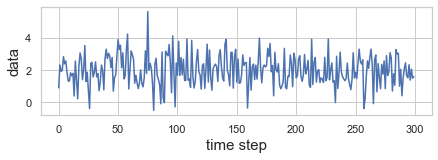
\includegraphics[width=\linewidth]{anomaly/figs/s1.png}
  \caption{Special Case I: stationary stream}
  \label{fig:s71}
\end{subfigure}%
\begin{subfigure}{.45\columnwidth}
  \centering
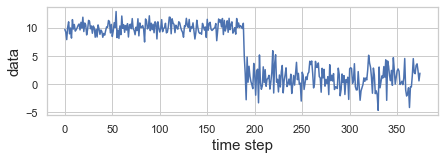
\includegraphics[width=\linewidth]{anomaly/figs/s2.png}
  \caption{Special Case II: distribution shift }
  \label{fig:s72}
\end{subfigure} \\
\begin{subfigure}{.45\columnwidth}
  \centering
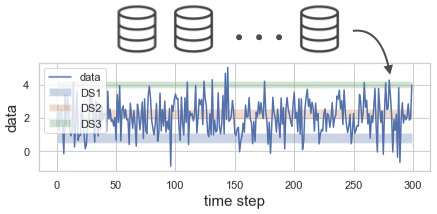
\includegraphics[width=\linewidth]{anomaly/figs/s3.jpeg}
  \caption{Special Case III: offline dataset }
\end{subfigure}%
\begin{subfigure}{.45\columnwidth}
  \centering
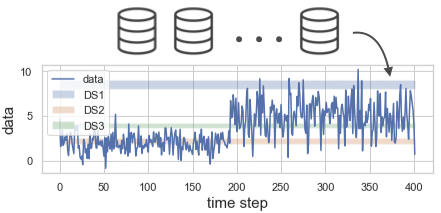
\includegraphics[width=\linewidth]{anomaly/figs/s4.jpeg}
  \caption{The General Case}
\end{subfigure}%
\caption{Illustration of the cases we study in this paper.}
\label{fig:setting_illustrations}
\end{figure}


\begin{figure}[h!]
    \centering
    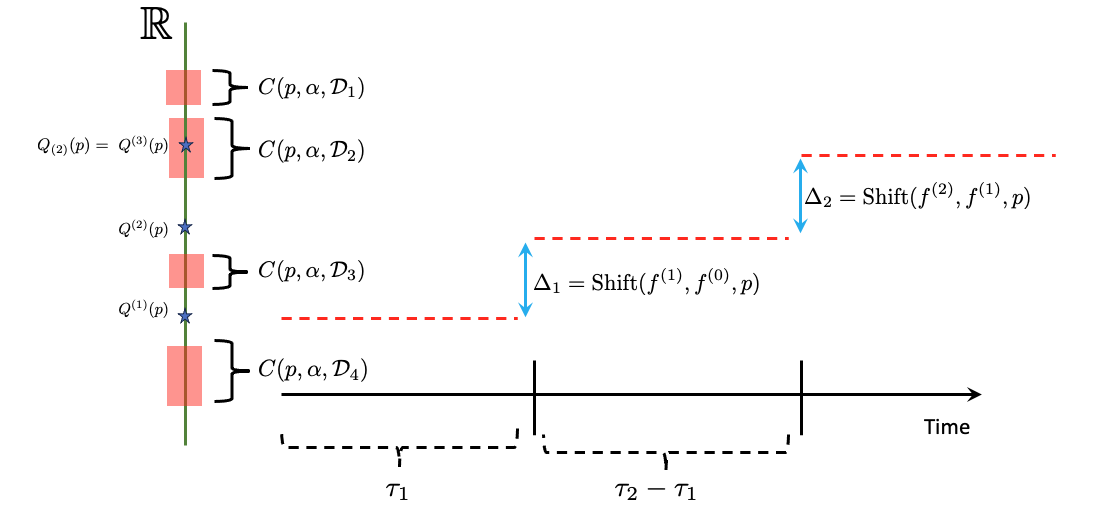
\includegraphics[width=0.8\linewidth]{anomaly/figs/separated_datasets.png}
    \caption{An illustration of Assumption \ref{asumption_detectable} and \ref{defn:offline_datasets} on a stream with $2$ change-points ($H_T=2)$ and $K=4$ offline datasets. Assumption \ref{asumption_detectable} implies that the change-points on the stream are sufficiently far apart. Assumption \ref{defn:offline_datasets} implies that the $4$ CS do not intersect. Moreover, either the true quantile on the stream are outside the offline CS, i.e., $Q^{(1)}(p)$ and $Q^{(2)}(p)$ are not contained in any offline dataset's CS. Or, it is the case that the online quantile matches one of the offline dataset, i.e., $Q_{(2)}(p) = Q^{(3)}(p)$ in this example.}
    \label{fig:separated_datasets_example}
\end{figure}

\pagebreak

\section{Proof of Theorem \ref{the:iid}, stationary setting}

\begin{algorithm}
\caption{OAD for stationary i.i.d. stream}\label{alg:one}
\SetKwInOut{Input}{Input}
\SetKwInOut{Output}{Output}
\Input{Quantile $p$, Confidence $1-\alpha$}
\Output{Anomaly labels $\hat{y}_1, \hat{y}_2, \ldots$}
\For{  $\text{each time }t \geq 1$ } {
    Receive $t^{th}$ input $S_t$\;
    
    Compute $C(p,\alpha, S_{1:t})$ (Eq. \ref{eq:cs})\;

    $\hat{y}_t \gets \text{{\ttfamily Algorithm }\ref{alg:marginal_decision}}(S_t, C(p,\alpha, S_{1:t}))$ \;
    
  %   %Compute $ub_t \gets \hat{Q}_t(p + u_t)$(Eq. \ref{eq:cs})\; 
  %   \uIf{$S_t > \max C(p,\alpha, S_{1:t})$}{
  %   $\hat{y}_t \gets1$\; \tcp{Declare an anomaly}
  % }
  % \uElseIf{$S_t \in C(p,\alpha , S_{1:t}$}{
  % $\hat{y}_t \gets * $ \; \tcp{Abstain from decision}
  % }
  % \Else{
  %   $\hat{y}_t \gets 0 $ \; \tcp{Declare benign}
  % }
}
\end{algorithm}

\begin{theorem}[Formal version of Theorem \ref{the:iid}]
If the data-source $S_1, S_2, \cdots$ are i.i.d., then with probability at-least $1-2\alpha$, for all times $T \in \mathbb{N}$, Algorithm \ref{alg:one} satisfies \begin{enumerate}
    \item $0$ False positives, $0$ False negatives
    \item Abstains is less than or equal to $7 \sqrt{T \ln \left( \frac{1612\ln(eT)}{\alpha^2} \right)}$,
    \item Abstains is at-least $\frac{1}{4} \sqrt{T \ln \left( \frac{1612\ln(eT)}{\alpha^2} \right)}$
    
\end{enumerate}
\label{the:iid_plus}
\end{theorem}
 
\begin{proof}
In order to give the proof, we set some notations. 

%
\begin{definition}[Good event $\gE_1$] %Denote the good event $\mathcal{E}_1$ as 
\begin{align}
\begin{split}
    \mathcal{E}_1 := \bigcap_{t \in \mathbb{N}} \bigcap_{p \in (0,1)} 
 \{  \widehat{Q}(p-u_t(\alpha), S_{1:t}) \leq Q(p) \leq \widehat{Q}(p+u_t(\alpha), S_{1:t}) \} .
\end{split}
\label{eqn:good_event_defn}
\end{align}   
\end{definition}
\vspace{-0.5em}
%
In words, the good event states that for all time $t$, the confidence sequence contains the true $p$th quantile.
From Corollary $2$ of \cite{howard2022sequential}, we know that $\mathbb{P}[\mathcal{E}] \geq 1-\alpha$. We remark that \cite{howard2022sequential} show that even when $(S_t)_{t \geq 1}$ are independent, but not necessarily identical, $\mathbb{P}[\mathcal{E}] \geq 1-\alpha$ holds as long as the $p$th quantile $Q_t(p) := Q(p)$ for all $t \geq 1$. This extension relaxing the identical distribution will be crucial in the subsequent sections in the sequel. 

Further, observe from the definition in Algorithm \ref{alg:one} and Equation (\ref{eq:cs}) that for all $t\in \mathbb{N}$ and $p \in (0,1)$,
\begin{align*}
     \{  \widehat{Q}(p-u_t(\alpha), S_{1:t}) \leq Q(p) \leq \widehat{Q}(p+u_t(\alpha), S_{1:t}) \} \subseteq \{ Q(p) \in C(p,\alpha, S_{1:t} \}.
\end{align*}

The reason for this inclusion is that the definition of $C(\cdot)$ in Equation (\ref{eq:cs}) has an extra factor of $2$, i.e., 
\begin{align*}
    C(p,\alpha,S_{1:t}) :=  \bigg[ \widehat{Q}(p- 2u_{n}(\alpha), y_{1:n}),  \widehat{Q}(p+2u_{n}(\alpha), y_{1:n}) \bigg].
\end{align*}


% Recall the good event $\mathcal{E}$ as defined in equation \ref{eqn:good_event_defn}.
% \begin{align*}
%     \mathcal{E} := \bigcap_{t \in \mathbb{N}} \bigcap_{p \in (0,1)} \{ Q(p) \leq \widehat{Q}_t(p+u_t) \} \bigcap \{ Q(p) \geq \widehat{Q}_t(p-u_t) \}.
% \end{align*}
% From Corollary $2$ of \cite{howard2022sequential}, we know that $\mathbb{P}[\mathcal{E}] \geq 1-\alpha$. 

In the rest of this proof, we will assume that the good event $\mathcal{E}$ holds. It is immediately clear the following two claims hold, proving the first two statements of the theorem.
\begin{claim}
If event $\mathcal{E}$ holds, then Algorithm 1 will not make any False Positive or False negative detections.
\label{claim:goodevent1}
\end{claim}

It now only remains to prove the third condition of the theorem. Define the sequence of indicator random variables indicating if time $t$ is an abstain
\begin{align} 
    Z_t := \mathbf{1}(\widehat{y}_t = *) .
\end{align} 

From Algorithm \ref{alg:one}, this is equivalent to 
\begin{align*}
    Z_{t} = \mathbf{1}(S_{t} \in (\widehat{Q}_t(p-2u_{t-1}(\alpha), S_{1:t-1}), \widehat{Q}_t(p+2u_{t-1}(\alpha), S_{1:t-1})).
\end{align*}
We denote by the filtration $(\mathcal{F}_t)_{t=1}^T$ to be generated by the observed sequence $(S_t)_{t=1}^T$, i.e., for all $t \in \{1,\cdots,T\}$, $\mathcal{F}_t := \sigma(S_1,\cdots,S_t)$. 


The proof of claim \ref{claim:goodevent1} follows from the following three lemmas. For clarity, proof for these lemmas can be found after this proof finishes.
 
% \begin{lemma}[Expectation of abstains] For every $t\geq2$, we have $\E(Z_t) \leq 3u_{t-1}(\alpha)$.
% \label{lem:exp_z}
% \end{lemma}

\begin{lemma}[Conditional expectation of abstains]
For every $ t \geq 2$, $$4u_{t-1}(\alpha) \leq \E[Z_t \mathbf{1}_{\mathcal{E}}| \mathcal{F}_{t-1}] \leq 6u_{t-1}(\alpha),$$ holds almost-surely.  
\label{lem:cond_exp}
\end{lemma}

\begin{lemma}[Azuma-Hoefding bound] 
Let $(Z_t)_{t=1}^T$ are bounded binomial variables and the sequence $(\mathcal{F}_t)_{t=1}^T$ is a probability filtration. Then for all $\varepsilon > 0$,
\begin{align*}
    \mathbb{P} \left[ \bigg| \sum_{s=1}^T Z_s  - \mathbb{E}[Z_s  \vert \mathcal{F}_{s-1}] \bigg| \geq \varepsilon \right] \leq 2 \exp \left( -\frac{ \varepsilon^2}{2T} \right)
\end{align*}
\label{lemma:azuma}
\end{lemma}

We now apply Lemma \ref{lemma:azuma} to the sequence of binary random variables $(\widetilde{Z}_t)_{t\geq 1} := (Z_t \mathbf{1}_{\mathcal{E}})_{t \geq 1}$ by setting $\varepsilon =  \sqrt{T \ln \left( \frac{4}{\alpha^2} \right)}$. Thus, with probability at least $1-\alpha$ %? $1-\frac{\alpha}{2}$
, we have

\begin{align*}
  \mathbb{P} \left[ \underbrace{ \bigg| \mathbf{1}_{\mathcal{E}} \sum_{s=1}^TZ_s - \sum_{s=1}^T \mathbb{E}[Z_s \mathbf{1}_{\mathcal{E}} \vert \mathcal{F}_{s-1}] \bigg| \leq   \sqrt{T \ln \left( \frac{4}{\alpha^2} \right)}}_{\text{Event } \mathcal{G}_1} \right] \geq 1- \alpha
  \end{align*}
  
From a simple union-bound argument, we see that $\mathbb{P}[\mathcal{E} \cap \mathcal{G}_1] \geq 1 - 2\alpha$. Furthermore by definition of event $\mathcal{G}_1$,  the following inequality holds almost-surely. 
\begin{align*}
    \mathbf{1}_{\mathcal{G}}\mathbf{1}_{\mathcal{E}_1} \sum_{s=1}^TZ_s &\leq \mathbf{1}_{\mathcal{G}_1}\left(\sum_{s=1}^T \mathbb{E}[Z_s \mathbf{1}_{\mathcal{E}} \vert \mathcal{F}_{s-1}] +  \sqrt{T \ln \left( \frac{4}{\alpha^2} \right)}\right),\\
        &\stackrel{\text{Lem } \ref{lem:cond_exp}}{\leq}  \mathbf{1}_{\mathcal{G}_1}\left( \sum_{t=1}^T 6u_{t-1}(\alpha) + \sqrt{T \ln \left( \frac{4}{\alpha^2} \right)}\right), \\
    &\stackrel{}{\leq}  \mathbf{1}_{\mathcal{G}_1}\left(6\sqrt{T \ln \left( \frac{1612 \ln(eT)}{\alpha} \right)} + \sqrt{T \ln \left( \frac{4}{\alpha^2} \right)}\right), \\
   &\leq  \mathbf{1}_{\mathcal{G}_1}\left(7\sqrt{T \ln \left( \frac{1612 \ln(eT)}{\alpha^2} \right)}\right).
\end{align*}
In other words, the preceding display reads that on the event $\mathcal{E} \cap \mathcal{G}_1$ holds, we have
  \begin{align*}
   \sum_{s=1}^TZ_s \leq 7\sqrt{T \ln \left( \frac{1612 \ln(eT)}{\alpha^2} \right)}.
\end{align*}
Similarly, from the definition of $\mathcal{G}_1$, we also have 
\begin{align*}
     \mathbf{1}_{\mathcal{G}}\mathbf{1}_{\mathcal{E}_1} \sum_{s=1}^TZ_s &\geq \mathbf{1}_{\mathcal{G}_1}\left(\sum_{s=1}^T \mathbb{E}[Z_s \mathbf{1}_{\mathcal{E}} \vert \mathcal{F}_{s-1}] -  \sqrt{T \ln \left( \frac{4}{\alpha^2} \right)}\right),\\
             &\stackrel{\text{Lem } \ref{lem:cond_exp}}{\geq}  \mathbf{1}_{\mathcal{G}_1}\left( \sum_{t=1}^T 2u_{t-1}(\alpha) - \sqrt{T \ln \left( \frac{4}{\alpha^2} \right)}\right), \\
    &\stackrel{}{\geq}  \mathbf{1}_{\mathcal{G}_1}\left(2\sqrt{T \ln \left( \frac{1612 \ln(eT)}{\alpha} \right)} - \sqrt{T \ln \left( \frac{4}{\alpha^2} \right)}\right), \\
   &\geq  \mathbf{1}_{\mathcal{G}_1}\left(\frac{1}{4}\sqrt{T \ln \left( \frac{1612 \ln(eT)}{\alpha^2} \right)}\right).
\end{align*}
The proof is complete since $\mathbb{P}[\mathcal{E} \cap \mathcal{G}_1] \geq 1-2\alpha$. 
\end{proof}


Below we provide the proof of each lemma used in proof of Theorem \ref{the:iid}. 

% \begin{proof}[Proof of Lemma \ref{lem:exp_z}]
% Note that again $\hat{Q}_t$ is the empirical quantile function of $\{S_i\}_{i=1}^{t-1}$. By exchangeability of i.i.d. samples, we know that the the probability of $S_t$'s rank among $\{S_i\}_{i=1}^{t-1}$ is uniform. Therefore,
% \begin{align*}
% \E(Z_t) = \prob (S_t \in [\hat{Q}(p-u_{t-1}(\alpha), S_{1:t-1}),\hat{Q}(p+u_{t-1}(\alpha),S_{1:t-1})])  \leq \frac{\ceil{2u_{t-1}(\alpha)\cdot (t-1)}}{t}  \leq  3u_t
% \end{align*}
% \end{proof}


\begin{proof}[Proof of Lemma \ref{lem:cond_exp}]
% In order to prove this result, we use the stornger Corollary $2$ of \cite{howard2022sequential}. We know from that corollary that if $g_t := 0.85\sqrt{t^{-1}(\log \log(et) + 0.8 \log (1612/\alpha))}$, then $$ \mathbb{P}[ \exists t \in \mathbb{N}, \exists p \in (0,1) : \{ Q(p) < \widehat{Q}_t(p-g_t) \} \cup  \{ Q(p) > \widehat{Q}_t(p + g_t) \} ] \leq  \alpha. $$
% Then in particular, we have
% {\color{black}
% \begin{align*}
%     \mathbb{P} \left[ \forall t, \{ Q(p+2u_t) \geq \widehat{Q}_t(p+u_t) \} \cap \text{  } \{ Q(p-2u_t) \leq \widehat{Q}_t(p-u_t) \} \right] \geq 1-\alpha. 
% \end{align*}
% }
% Thus, 
We can compute the conditional expectation as 
\begin{align*}
    \E[Z_t \mathbf{1}_{\mathcal{E}}| \mathcal{F}_{t-1}] 
    &= \mathbb{P}[S_t \in (\widehat{Q}(p-2u_{t-1}(\alpha),S_{1:t-1}), \widehat{Q}(p+2u_{t-1}(\alpha),S_{1:t-1}) ) \cap \mathcal{E} \vert \mathcal{F}_{t-1}], \\
        &\stackrel{(a)}{\leq}  \mathbb{P}[S_t \in (Q(p-3u_{t-1}(\alpha)), Q(p+3u_{t-1}(\alpha)) \vert \mathcal{F}_{t-1}]  \\
        &\stackrel{(b)}{\leq}  \mathbb{P}[S_t \in (Q(p-3u_{t-1}(\alpha)), Q(p+3u_{t-1}(\alpha)) ]  \\
    & \stackrel{(c)}{\leq} 6u_{t-1}(\alpha).
\end{align*}
Step $(a)$ follows from the fact that on event $\mathcal{E}$, for all times $t \in \mathbb{N}$ and quantiles $p \in (0,1)$, we have $Q(p) \leq \widehat{Q}(p+u_t(\alpha),S_{1:t})$ and $Q(p) \geq \widehat{Q}(p-u_t(\alpha),S_{1:t-1})$ holds. Step $(b)$ follows since $(S_t)_{t \geq 1}$ is an i.i.d. sequence and thus $S_t$ is independent of $\mathcal{F}_{t-1}$. Step $(c)$ follows from the standard fact the for any $\mathbb{R}$ valued continuous random variable, and for any quantiles $0 \leq p_1 \leq p_2 \leq 1 $, $\mathbb{P}[X \in (Q(p_1), Q(p_2))] = p_2 - p_1$.
Similarly, we have 
\begin{align*}
    \E[Z_t \mathbf{1}_{\mathcal{E}}| \mathcal{F}_{t-1}] 
    &= \mathbb{P}[S_t \in (\widehat{Q}(p-2u_{t-1}(\alpha),S_{1:t-1}), \widehat{Q}(p+2u_{t-1}(\alpha),S_{1:t-1}) ) \cap \mathcal{E} \vert \mathcal{F}_{t-1}], \\
        &\stackrel{(a)}{\geq}  \mathbb{P}[S_t \in (Q(p-u_{t-1}(\alpha)), Q(p+u_{t-1}(\alpha)) \vert \mathcal{F}_{t-1}]  \\
        &\stackrel{(b)}{\leq}  \mathbb{P}[S_t \in (Q(p-u_{t-1}(\alpha)), Q(p+u_{t-1}(\alpha)) ]  \\
    & \stackrel{(c)}{\leq} 2u_{t-1}(\alpha).
\end{align*}
follows from the fact that on event $\mathcal{E}$, for all times $t \in \mathbb{N}$ and quantiles $p \in (0,1)$, we have $Q(p) \leq \widehat{Q}(p+u_t(\alpha),S_{1:t})$ and $Q(p) \geq \widehat{Q}(p-u_t(\alpha),S_{1:t-1})$ holds. Step $(b)$ follows since $(S_t)_{t \geq 1}$ is an i.i.d. sequence and thus $S_t$ is independent of $\mathcal{F}_{t-1}$. Step $(c)$ follows from the standard fact the for any $\mathbb{R}$ valued continuous random variable, and for any quantiles $0 \leq p_1 \leq p_2 \leq 1 $, $\mathbb{P}[X \in (Q(p_1), Q(p_2))] = p_2 - p_1$.
\end{proof}

\begin{proof}[Proof of Lemma \ref{lemma:azuma}]
Denote by the sequence of $0$ mean random variables $\widetilde{Z}_t := Z_t - \mathbb{E}[Z_t \vert \mathcal{F}_{t-1}]$. Denote by the running sum $Y_t := \sum_{s=1}^{t} \widetilde{Z}_s$. It is easy to verify that $(Y_t)_{t=1}^T$ is a martingale sequence. Further from definition, we have have that almost-surely, for all $t \in \{1,\cdots, T\}$, $|Y_{t} - Y_{t+1}| \leq 2$. Thus, from Azuma Hoeffding inequality for bounded martingales, we have that 
\begin{align}
    \mathbb{P}\left[\sum_{s=1}^T \widetilde{Z}_s \geq \sqrt{T \ln \left( \frac{4}{\alpha^2} \right)}\right] &\leq 2 \exp \left( - \frac{2 T \ln \left( \frac{4}{\alpha^2} \right)}{4T} \right), \\
    &\leq \frac{\alpha}{2}.
\end{align}


\end{proof}

\section{Proofs from Section \ref{sec:offline-only}}



The proofs in this section are dependent on the following good-event, under which we will perform the analysis.

%\subsection{Good events for quantile estimation}

\begin{definition}[Good event 2] 
Let $(S_t)_{t=1}^T \sim \Bigl(T,H_T, (\tau_c)_{c=0}^{H_T}, (f^{(c)})_{c=0}^{H_T}\Bigr)$, with quantile functions of the $H_T+1$ segments given by $(Q^{(c)}(\cdot))_{c=0}^{H_T}$. Define $\gE_2$ as
\begin{align}
    \widehat{\gE_2} := \bigcap_{k=1}^{H_T} \gE_2^{(k)},
    \label{eqn:good_event_2_defn_internal}
\end{align}
where for each $k \in [H_T]$, 
\begin{align*}
        \mathcal{E}_2^{(k)} =  \bigcap_{p \in [0,1]} \bigcap_{t_1 = \tau_{k}}^{\tau_{k+1}} \bigcap_{t_2 = t_1 +1}^{\tau_{k+1}}   \bigg\{ \widehat{Q}(p-u_{t_2 - t_1}(\alpha), S_{t_1:t_2})  \leq Q^{(k)}(p) \leq \widehat{Q}(p-u_{t_2 - t_1}(\alpha), S_{t_1:t_2}) \bigg\},
\end{align*}
where $\widehat{Q}$ is the empirical quantile and $u_{(\cdot)}(\cdot)$ is defined in Equation (\ref{eqn:defn_confidence_width_ut}).
\label{as:goodevent2}
\end{definition}
%\vspace{-1em}
%
In words,  $\gE_2$ is the intersection over all the $H_T+1$ stationary segments, where for each segment the quantile estimate is close to the true quantile for all quantiles. Following Corollary $2$ of \cite{howard2022sequential} and an union bound, we get the following.

\begin{proposition}
    \begin{align*}
        \mathbb{P}[\widehat{\gE_2}] \geq 1 - T\alpha.
    \end{align*}
    \label{prop:good_event_2_prob_hat}
\end{proposition}
\begin{proof}
    We analyze the complement as follows.
    \begin{align*}
        & \quad \; \mathbb{P}[\widehat{\gE_2}^{\complement}] \\ &= \mathbb{P} \left[ \cup_{k=0}^{H_T} \cup_{p \in [0,1]} \cup_{t_1=\tau_k}^{\tau_{k+1}} \cup_{t_2 \geq t_1 + 1} \{ \widehat{Q}(p-u_{t_2 - t_1}(\alpha), S_{t_1:t_2})  > Q^{(k)}(p) \} \cup \{ Q^{(k)}(p) > \widehat{Q}(p-u_{t_2 - t_1}(\alpha), S_{t_1:t_2}) \}  \right], \\
        &\leq \sum_{k=0}^{H_T} \sum_{t_1=\tau_k}^{\tau_{k+1}}\mathbb{P} \left[ \cup_{p \in [0,1]} \cup_{t_2 \geq t_1 + 1} \{ \widehat{Q}(p-u_{t_2 - t_1}(\alpha), S_{t_1:t_2})  > Q^{(k)}(p) \} \cup \{ Q^{(k)}(p) > \widehat{Q}(p-u_{t_2 - t_1}(\alpha), S_{t_1:t_2}) \}  \right], \\
        &\stackrel{(a)}{\leq}\sum_{k=0}^{H_T} \sum_{t_1=\tau_k}^{\tau_{k+1}}\alpha, \\
        &= T \alpha.
    \end{align*}
    Step $(a)$ follows from   Corollary $2$ of \cite{howard2022sequential}.
\end{proof}

{\color{black}

In addition, we also need a generalization of event $\mathcal{G}_1$ to the piece-wise stationary stream. 

\begin{align}
  \gG_2:=  \bigcap_{k=0}^{H_T} \bigcap_{t_1 = \tau_k + 1}^{\tau_{k+1}}\bigg\{ \bigg| \sum_{t=t_1}^{\tau_{k+1}}Z_{t:t_1} - \mathbb{E}[Z_{t:t_1} \vert \mathcal{F}_{t-1}] \bigg| \leq \sqrt{(\tau_{k+1} - \tau_k) \ln \left( \frac{4}{\alpha^2} \right)} \bigg\},
  \label{eqn:good_event_G}
\end{align}
where 
\begin{align}
    Z_{t:t_1} := \mathbf{1}(S_{t} \in (\widehat{Q}_t(p-2u_{t-t_1}(\alpha), S_{t_1:t-1}), \widehat{Q}_t(p+2u_{t-t_1}(\alpha), S_{t_1:t-1})),
\end{align}
and $\mathcal{F}_{t-1} := \sigma(S_{1:t-1})$ is the sigma-algebra generated by the first $t-1$ samples.

\begin{proposition}
    \begin{align*}
        \mathbb{P}[\gG_2] \geq 1 - T \alpha.
    \end{align*}
    \label{prop:abstain_good_event}
\end{proposition}
For a given $k$ and $t_1$, the proof follows from an application of Azuma-Hoeffding similar to the proof of Theorem \ref{the:iid}. Applying an union bound over $k$ and $t_1$ yields the result. 

In the rest of this section, denote the good event $\gE_2$ as 
\begin{align}
    \gE_2 = \widehat{\gE_2} \bigcap \gG_2,
    \label{eqn:good_event_2_defn}
\end{align}
where $\widehat{\gE}_2$ is defined in Equation (\ref{eqn:good_event_2_defn_internal}) and $\gG_2$ in Equation (\ref{eqn:good_event_G}).

\begin{proposition}
    \begin{align*}
        \mathbb{P}[\widehat{\gE_2}] \geq 1 - T\alpha.
    \end{align*}
    \label{prop:good_event_2_prob}
\end{proposition}
The proof follows from an union bound using estimates in Proposition \ref{prop:good_event_2_prob_hat} and \ref{prop:abstain_good_event}.

}

\subsection{Proof of Proposition \ref{prop:delay_bound}}


\begin{figure}[h!]
    \centering
    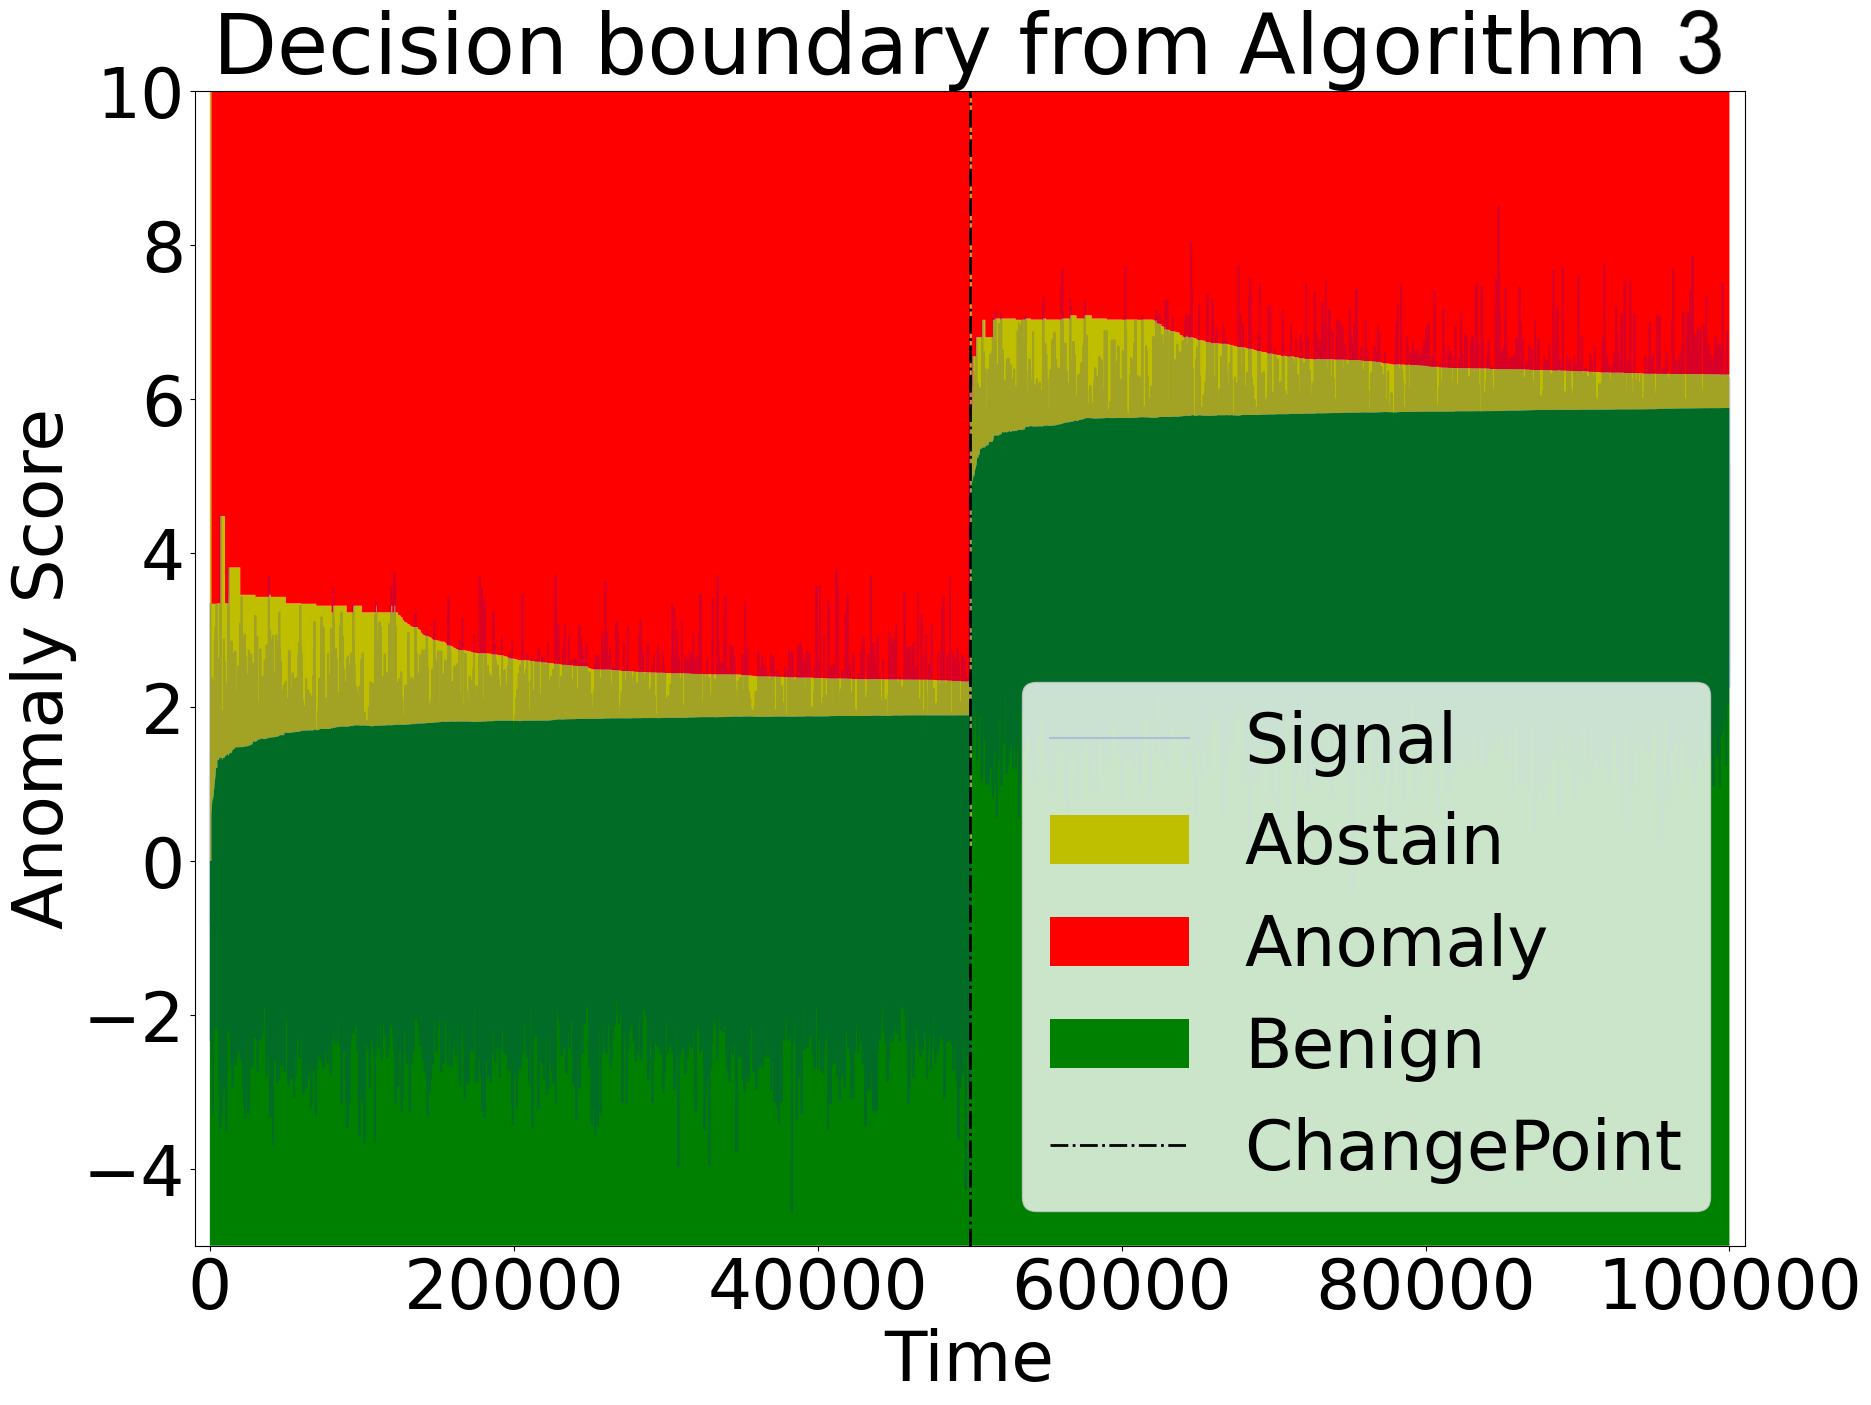
\includegraphics[width=0.4\linewidth]{anomaly/figs/algo_2_example.png}
    \caption{Algorithm 3 output on a piece-wise stationary stream.}
    \label{fig:s1}
\end{figure}

In order to give the proof of Proposition \ref{prop:delay_bound}, we need the following general lemma on change-detection. 


\begin{proposition}[Stream with a single change-point]
Let $(S_t)_{t=1}^T$ be a piecewise stationary stream with a single change-point, i.e., $H_T = 1$ with the change-point instant $\tau_1 = \tau \in [T]$. Denote by $\Delta := \text{Shift}(f^{(0)}, f^{(1)}, p)$ as the distribution shift magnitude. Denote by $\tau' \in \mathbb{N}$ as the first time when the {\ttfamily if} statement in Algorithm \ref{alg:two} evaluates to {\ttfamily True}, i.e., a change is detected for the first time by Algorithm \ref{alg:two}. Then, under the good event  $\gE_2$  (Definition \ref{as:goodevent2}), 
\begin{align*}
    \tau \leq \tau' 
    &\leq \bigg\lceil \inf_{\widetilde{\tau}} \left\{  u_{\tau}(\alpha) + u_{\widetilde{\tau}-\tau}(\alpha) \leq \frac{\Delta}{6} \right\} \bigg\rceil,
\end{align*}
where $u_t(\alpha)$ is given in Equation (\ref{eqn:defn_confidence_width_ut}). 
\label{prop:dist_changes}
\end{proposition}


We recall some notation to give the proof. The two distributions are denoted by $f^{(0)}$ and $f^{(1)}$ and their corresponding quantile functions are given by $Q^{(0)}(\cdot)$ and $Q^{(1)}(\cdot)$, where for $i \in \{0,1\}$, the function $Q^{(i)}(\cdot) : [0,1] \to \mathbb{R}$ is such that for all $p \in [0,1]$, $Q^{(i)}(p)$ is the $p$th quantile of the distribution $f^{(i)}$. Since we assume all distributions are continuous, the existence and uniqueness of quantile functions are granted. 

\textbf{Proof that $\tau \leq \tau'$}

Observe that under the event $\gE_2$, we have for all $t_1 < t_2 \in [\tau]$, $Q^{(0)}(p) \in C(p,\alpha, S_{t_1:t_2})$. Thus, for all $t \in [\tau]$, $Q^{(0)}(p) \in \bigcap_{s=1}^t C(p,\alpha,S_{s:t}) \bigcap_{s=1}^t C(p,\alpha,S_{1:s})$, and in particular, $\bigcap_{s=1}^t C(p,\alpha,S_{s:t}) \bigcap_{s=1}^t C(p,\alpha,S_{1:s})$ is non-empty. Therefore, under event $\gE_2$, for all $t \in [\tau]$, Algorithm \ref{alg:change_point} will never return {\ttfamily True} for the input sequence $S_{1:t}$.

\textbf{Proof on the upper bound of $\tau'$}

Since $\Delta > 0$, we will assume here that $Q^{(0)}(p) < Q^{(1)}(p)$ and this is without loss of generality since the proof for the other case follows identically. 
To prove the upper bound, it suffices to prove that if event $\gE_2$ holds and no change is detected till time $\tau' = \inf \{\widetilde{\tau}: u_{\tau}(\alpha)+ u_{\widetilde{\tau}-\tau}(\alpha) \}$, then at time $\lceil \tau' \rceil$, a change point will be detected. 

In order to prove this, we need to establish that $\bigcap_{s=1}^{\lceil \tau' \rceil} C(p,\alpha,S_{s:t}) \bigcap_{s=1}^{\lceil \tau' \rceil} C(p,\alpha,S_{1:s}) = \emptyset$. A sufficient condition for this is to prove that $C(p,\alpha,S_{\tau+1:\lceil \tau' \rceil}) \bigcap C(p,\alpha,S_{1:\tau}) = \emptyset$, i.e., the following implication holds 
\begin{align}
    C(p,\alpha,S_{\tau+1:\lceil \tau' \rceil}) \bigcap C(p,\alpha,S_{1:\tau}) = \emptyset \implies \bigcap_{s=1}^{\lceil \tau' \rceil} C(p,\alpha,S_{s:t}) \bigcap_{s=1}^{\lceil \tau' \rceil} C(p,\alpha,S_{1:s}) = \emptyset.
    \label{eqn:setting_2_internal_implication}
\end{align}
From Equation (\ref{eq:cs}), we know that 
\begin{align*}
     C(p,\alpha,S_{1:\tau}) = \bigg[ \widehat{Q}(p-2u_{\tau}(\alpha), S_{1:\tau}), \widehat{Q}(p+2u_{\tau}(\alpha), S_{1:\tau}) \bigg].
\end{align*}

Since event $\gE_2$ holds, it follows that 
\begin{align}
    \widehat{Q}(p+2u_{\tau}(\alpha),S_{1:\tau}) &\leq Q^{(0)}(p+3u_{\tau}(\alpha))     \label{eqn:setting_2_delay_pf_11}\\
    \widehat{Q}(p-2u_{\lceil \tau' \rceil - \tau}(\alpha)) &\geq Q^{(1)}(p - 3u_{\lceil \tau' \rceil-\tau}(\alpha)).
    \label{eqn:setting_2_delay_pf_1}
\end{align}
Further, from the definition of $\Delta$ in Definition \ref{def:quantile_shift} and the assumption that $Q^{(0)}(p) < Q^{(1)}(p)$ we know that 
\begin{align}    
Q^{(0)}( p + {\Delta} ) \leq Q^{(1)}(p - {\Delta})
    \label{eqn:setting_2_delay_pf_2}
\end{align}

Now, from the definition of $\tau'$, we know that 
\begin{align}
    3(u_{\tau}(\alpha) + u_{\lceil {\tau'} \rceil-\tau}(\alpha)) \leq {\Delta}
        \label{eqn:setting_2_delay_pf_3}
\end{align}

Now, combining the inequalities in Equations (\ref{eqn:setting_2_delay_pf_1}, \ref{eqn:setting_2_delay_pf_2}, \ref{eqn:setting_2_delay_pf_3}), we get that 
\begin{multline}
\widehat{Q}(p+2u_{\tau}(\alpha),S_{1:\tau}) \stackrel{\ref{eqn:setting_2_delay_pf_11}}{\leq} Q^{(0)}(p+3u_{\tau}(\alpha)) \stackrel{(a)}{<} Q^{(0)}(p+3u_{\tau}(\alpha) + 3u_{\lceil {\tau'} \rceil-\tau}(\alpha)) \stackrel{\ref{eqn:setting_2_delay_pf_3}}{\leq} Q^{(0)}(p+{\Delta}) \stackrel{\ref{eqn:setting_2_delay_pf_2}}{\leq} \\ Q^{(1)} ( p - {\Delta} ) \stackrel{\ref{eqn:setting_2_delay_pf_3}}{\leq} Q^{(1)}(p-3u_{\lceil {\tau'} \rceil-\tau}(\alpha)) \stackrel{\ref{eqn:setting_2_delay_pf_1}}{\leq} \widehat{Q}(p-2u_{\tau}(\alpha),S_{\tau:\lceil {\tau'} \rceil}).
\label{eqn:disjoint}
\end{multline}
Step $(a)$ follows from the fact that since $f^{(0)}$ and $f^{(1)}$ are a continuous distribution, we have for all $i \in \{0,1\}$ and a;; $0 < p_1 < p_2 < 1$, $Q^{(i)}(p_1) < Q^{(i)}(p_2)$. Thus, Equation (\ref{eqn:disjoint}) gives that under the event $\gE_2$, $   C(p,\alpha,S_{\tau+1:\lceil \tau' \rceil}) \bigcap C(p,\alpha,S_{1:\tau}) = \emptyset$, which from Equation (\ref{eqn:setting_2_internal_implication}) implies that if Algorithm \ref{alg:change_point} is queried with input $S_{1:\lceil \tau' \rceil}$, will return a {\ttfamily 1}, i.e., detect a change-point.


\textbf{Concluding the proof of Proposition \ref{prop:delay_bound} as an application of Proposition \ref{prop:dist_changes}}

% \begin{proposition*}[\ref{prop:delay_bound}]
% If the number of pre-change samples $\tau \geq \frac{20}{\Delta^2}\ln \left( \frac{1612}{\alpha \Delta^2}\right)$, then $\text{Delay}(\tau, \Delta, \alpha) \leq \frac{20}{\Delta^2}\ln \left( \frac{1612}{\alpha \Delta^2}\right).$
% \end{proposition*}

\begin{proof}
% Let $\tau$ denote the number of pre-change samples, and let $\tau'$ denote the point where the changes are detected. Delay can be defined as $\tau' - \tau$.  Suppose $\tau \geq \frac{20}{\Delta^2}\ln \left( \frac{1612}{\alpha \Delta^2}\right)$.

% For a change of magnitude $\Delta$ with $\tau$ pre-change samples to be detectable under the good event $\gE_2$, a \emph{sufficient} condition is that the forward and backward confidence sequences becomes disjoint at time $\tau$:
% \begin{align}
%     2(u_{\tau}(\alpha) + u_{\tau'- \tau}(\alpha)) \leq \Delta
% \label{eq:detectability}
% \end{align}

The proof rests on the following numerical claim.

\begin{claim}
If $\tau \geq \frac{80}{\Delta^2}\ln \left( \frac{1612}{\alpha \Delta^2}\right)$, then $u_\tau(\alpha) \leq \Delta/6 $ holds.
\label{claim:delay1}
\end{claim}
{\color{black}
\begin{proof}[Proof of Claim \ref{claim:delay1}]
Suppose $\tau \geq \frac{80}{\Delta^2}\ln \left( \frac{1612}{\alpha \Delta^2}\right)$. Then
\begin{align*} 
    u_{\tau}(\alpha) &\leq \sqrt{\frac{\ln \left( \frac{1612}{\alpha}(1+\ln(\tau)) \right)}{\tau}}, \\
    &\leq \frac{\Delta}{6}  \frac{\sqrt{{\ln \left( \frac{1612}{\alpha}(1+\ln(\tau)) \right)}}}{\sqrt{5\ln \left( \frac{1612}{\alpha \Delta^2} \right)}}, \\
    &\leq \frac{\Delta}{6} \frac{\sqrt{\ln \left( \frac{1612}{\alpha}\left(1+\ln\left(\frac{20}{\Delta^2}\ln \left( \frac{1612}{\alpha \Delta^2} \right)\right)\right) \right)}}{{\sqrt{5\ln \left( \frac{1612}{\alpha \Delta^2} \right)}}}, \\
    &\leq \frac{\Delta}{6}.
\end{align*}
\end{proof}

Applying Claim 2 to both $\tau$ and $\tau' - \tau$ allows use to satisfy the condition in Proposition \ref{prop:delay_bound}.

\begin{align*}
    & \tau \geq  \frac{80}{\Delta^2}\ln \left( \frac{1612}{\alpha \Delta^2}\right), \; \lceil \tau' \rceil - \tau \geq  \frac{80}{\Delta^2}\ln \left( \frac{1612}{\alpha \Delta^2}\right) \\
\Longrightarrow \;\; & u_{{\tau}}(\alpha) \leq \Delta/6, \; u_{{\lceil \tau' \rceil-\tau}}(\alpha) \leq \Delta/6, \\
\Longrightarrow \;\; & 3(u_{{\tau}}(\alpha)+ u_{{\lceil \tau' \rceil-\tau}}(\alpha)) \leq \Delta
\end{align*}

%Note that  $\tau' = \tau + \text{Delay}(\tau, \Delta, \alpha)$; we obtain $\text{Delay}(\tau, \Delta, \alpha) \leq \frac{80}{\Delta^2}\ln \left( \frac{1612}{\alpha \Delta^2}\right)$ by substituting the result above.  
}
\end{proof}



\subsection{Proof of Theorem \ref{thm:online_shift}}

% \begin{theorem*}[ \ref{thm:online_shift}]
% Let $(S_t)_{t = 1}^T$ be generated from a piece-wise stationary process $\Bigl(T,H_T, (\tau_c)_{c=0}^{H_T}, (f_c)_{c=0}^{H_T}\Bigr)$ with quantile shifts  $\Delta_{k} := \text{Shift} (f_{k},f_{k+1})$, $\forall k \in [1,H_T]$. With probability at-least $1-T\alpha$, Algorithm \ref{alg:two} satisfies 
% \begin{itemize}
%     \item False positive and false negative satisfy 
%     \[\text{FP} + \text{FN}  \leq \sum_{k=1}^{H_T}D(\Delta_{k},\alpha) = H_t \cdot {\gO}(\frac{1}{(\Delta_{min})^2}) 
%     \]
%     \item Number of abstains less than 
%     \begin{align*}
%         \sum_{k=1}^{H_T} \Bigl[ &4 \sqrt{(\tau_k-\tau_{k-1}) \ln \left( \frac{1612}{\alpha^2} \ln(e(\tau_k-\tau_{k-1})) \right)} + D(\Delta_{k},\alpha) \Bigr]
%     \end{align*}
% \end{itemize}
% where $D(\Delta_{k},\alpha)$ is defined in Equation (\ref{eq:delay_shorthand}).
% \end{theorem*}

\begin{theorem*}[ \ref{thm:online_shift}]%[Bounds for setting 2, algorithm \ref{alg:two}]
Let $(S_t)_{t = 1}^T \sim \Bigl(T,H_T, (\tau_c)_{c=0}^{H_T}, (f_c)_{c=0}^{H_T}\Bigr)$ be  a piece-wise stationary data-stream satisfying Assumption \ref{asumption_detectable} for $\alpha \in (0,1)$. Then, with probability at-least $1-2T\alpha$, Algorithm \ref{alg:two} satisfies {\em both}
\begin{itemize}
    \item $\text{FP} + \text{FN}  \leq \sum_{k=1}^{H_T}D(\Delta_{k},\alpha) = H_T \cdot {\gO}(\frac{1}{(\min_k\Delta_{k})^2}) $, 
    \item Number of abstains $ \leq \sum_{k=1}^{H_T} \Bigl[ 7 \sqrt{(\tau_k-\tau_{k-1}) \ln \left( \frac{1612}{\alpha^2} \ln(3(\tau_k-\tau_{k-1})) \right)}  + D(\Delta_{k},\alpha) \Bigr]$,
\end{itemize}
where for all $k \in [H_T]$, $\Delta_{k} = \text{Shift} (f^{(k)},f^{(k-1)},p)$  is the quantile shift defined in Definition (\ref{def:quantile_shift}) and $D(\cdot,\cdot)$ is defined in Equation (\ref{eq:delay_shorthand}).
%\label{thm:online_shift}
\end{theorem*}




At a high-level, the proof idea is to show in Lemma \ref{lem:bdd_delay_change_induction} that if Assumption \ref{asumption_detectable} holds, then under the good event in Equation (\ref{eqn:good_event_2_defn}) {\em (i)} there are no false positive detections, and {\em (ii)} all the true changes are detected with bounded delay. This will conclude the proof of Theorem \ref{thm:online_shift} since a simple union bound over Corollary $2$ of \cite{howard2022sequential} implies that the good event in Equation (\ref{eqn:good_event_2_defn}) holds with probability at-least $1-T \alpha$.

In order to formalize the proof, we recall notations. As before, denote by $\tau_1 < \tau_2 \cdots < \tau_k < \tau_{k+1}$ be the set of times at which a true-change occurs. For each $k \in \{1, \cdots, H_T\}$, denote by $\tau'_k$ as the time at which Algorithm \ref{alg:two} detects a change for the $k$th time. The first observation is the lemma below which states that there are no false positives and the delay of all change detections are bounded.


% \begin{lemma}[No False Positives]
%      Under the event $\mathcal{E}_2$, $\tau_k^{'} \geq \tau_k$ holds for all $k \in \{1, \cdots, H_T\}$.
%      \label{lem:no_fp_in_change}
% \end{lemma}

\begin{lemma}[No false detections and bounded delay]
    Under the event $\mathcal{E}_2$, if Assumption \ref{asumption_detectable} holds, then for all $k \in \{1, \cdots, H_T\}$, 
    \begin{itemize}
        \item  $\tau'_k \geq \tau_k$, and
        \item $\tau'_k - \tau_k \leq D(\Delta_k, \alpha)$.
    \end{itemize}
    \label{lem:bdd_delay_change_induction}
\end{lemma}

Before giving the proof of the lemma, we show how it concludes the Proof of Theorem \ref{thm:online_shift}.

\begin{proof}[Proof of Theorem \ref{thm:online_shift}]
    
We can break down the analysis by change points, because we know that all changes are detected before the next change occurs. Moreover, Algorithm \ref{alg:two} restarts a fresh copy of Algorithm \ref{alg:one} after each change point is detected, and thus we can use the guarantees given in Theorem \ref{the:iid}.

Consider a subset of time points $[S_{\tau_k}, S_{\tau_{k+1}}]$ for some $ k\in[1,H_T]$. We will denote the time step of detecting change point $\tau_k$,  as $\tau'_k$.  The total number of mistakes (false positives and false negatives) is the sum of mistakes before and after $\tau'_k$. Therefore under the good event $\gE_2$ we have:

\begin{align*}
    \text{FP} + \text{FN} &= \sum_{k=0}^{H_T} \left( \sum_{t=\tau_k}^{\tau'_k} \mathbf{1}(\text{Time $t$ is a mistake)} + \sum_{t=\tau'_k + 1}^{\tau_{k+1}} \mathbf{1}(\text{Time $t$ is a mistake)} \right) \\
    %&\sum_{k=0}^{H_T}  [\text{mistakes}(S_{\tau_k:\tau'_k}) + \text{mistakes}(S_{\tau'_k:\tau_{k+1}})] \\ 
    &\leq \sum_{k=0}^{H_T} (\tau'_k - \tau_k) + 0 \quad \quad \text{(Event $\gE_2$ definition in Equation (\ref{eqn:good_event_2_defn}))}\\
    &\leq \sum_{k=0}^{H_T} D(\Delta_k, \alpha) + 0 \quad \quad \text{(Lemma \ref{lem:bdd_delay_change_induction})}\\
\end{align*}

%The last inequality follows since Lemma \ref{lem:bdd_delay_change_induction} gives that $\tau_k^{'} - \tau_k \leq D(\Delta_k, \alpha)$ and Theorem \ref{the:iid} gives that Algorithm \ref{alg:one} incurs no FP or FN under event $\mathcal{E}_1$. 
The analysis is similar for number of abstains. 
\begin{align*}
    \text{Abstains}  &= \sum_{k=0}^{H_T} \left( \sum_{t=\tau_k}^{\tau'_k} \mathbf{1}(\text{Time $t$ is abstained)} + \sum_{t=\tau'_k + 1}^{\tau_{k+1}} \mathbf{1}(\text{Time $t$ is abstained)} \right) \\
    %&= \sum_{k=0}^{H_T} [\text{abstains} (S_{\tau_k:\tau'_k}) + \text{abstains}(S_{\tau'_k:\tau_{k+1}})] \\
    &\leq \sum_{k=0}^{H_T} \left[(\tau_{k}' - \tau_k) + \sum_{t=\tau'_k + 1}^{\tau_{k+1}} \mathbf{1}(\text{Time $t$ is abstained)}\right] \\
    &\stackrel{\text{Lemma \ref{lem:bdd_delay_change_induction}}}{\leq} \sum_{k=0}^{H_T} 
    \Bigl[ D(\Delta_k, \alpha) + \sum_{t=\tau'_k + 1}^{\tau_{k+1}} \mathbf{1}(\text{Time $t$ is abstained)} \Bigr], \\
     &\stackrel{(a)}{\leq} \sum_{k=0}^{H_T} 
    \Bigl[ D(\Delta_k, \alpha) + \sum_{t=\tau_k' + 1}^{\tau_{k+1}} \mathbf{1}(Z_{t:\tau'_k}=1) \Bigr], \\
         &\stackrel{(b)}{\leq} \sum_{k=0}^{H_T} 
    \Bigl[ D(\Delta_k, \alpha) +  7 \sqrt{(\tau_k-\tau_{k-1}) \ln \left( \frac{1612}{\alpha^2} \ln(3(\tau_k-\tau_{k-1})) \right)}  \Bigr].
\end{align*}
In step $(a)$, we use the definition of $Z_{t:t_1}$ as used in Equation (\ref{eqn:good_event_G}) and in step $(b)$, we use the fact that event $\gG_2$ holds and thus the calculations from Theorem \ref{the:iid} can be used. 
\end{proof}

\subsection{Proofs of Lemma  \ref{lem:bdd_delay_change_induction}}

%\begin{proof}[Proof of Lemma \ref{lem:no_fp_in_change}]
We prove the result by induction on $k \in \{1,\cdots, H_T\}$. 

\textbf{Base case of $k=1$}: 
Observe that under event $\mathcal{E}_2$, we have $\tau_1^{'} \geq \tau_1$. This is so since for all times $t \in \{1,\cdots, \tau_1\}$, there will be no distribution-shift detected, since by definition under event $\mathcal{E}_2$, the forward and backward CS will contain at-least the true quantile and will thus be non-empty. 

Now, under Assumption \ref{asumption_detectable}, we know that $\tau_1 \geq \frac{20}{\Delta_1^2}\ln \left( \frac{1612}{\alpha \Delta_1^2}\right)$. Thus, by Proposition \ref{prop:delay_bound}, we know that $\tau_1^{'} - \tau_1 \leq \frac{20}{\Delta_1^2}\ln \left( \frac{1612}{\alpha \Delta_1^2}\right) := D(\Delta_1, \alpha)$, where the last equality is from  definition in Equation (\ref{eq:delay_shorthand}). This proves the induction base case. 

\textbf{Induction hypothesis}: Now, assume that for some $k \in \{1,\cdots, H_t\}$, we have that $\tau_{k}^{'} - \tau_k \leq D(\Delta_k, \alpha)$. We will now show that the $(k+1)$th detection time $\tau_{k+1}^{'}$ satisfies $\tau_{k+1}^{'} - \tau_{k+1} \leq D(\Delta_{k+1}, \alpha)$.

Assumption \ref{asumption_detectable} ensures that $\tau_{k+1} - \tau_{k} \geq D(\Delta_{k+1}, \alpha) + D(\Delta_k, \alpha)$. The induction hypothesis gives that  $\tau_{k}^{'} - \tau_k \leq D(\Delta_k, \alpha)$. Thus, under Assumption \ref{asumption_detectable} and the induction hypothesis,  we have that $\tau_{k+1} - \tau_k^{'} \geq D(\Delta_{k+1}, \alpha)$. From the working in Algorithm \ref{alg:two}, we know that at time $\tau_k^{'}$, a new instantiation of Algorithm \ref{alg:one} is started. Following the same arguments as for the base-case, we know that under the good-event $\mathcal{E}_2$, $\tau_{k+1}^{'} \geq \tau_{k+1}$, i.e., there are no false-positive detection. Moreover, since this re-started version of Algorithm \ref{alg:one} has seen at-least $\tau_{k+1} - \tau_k^{'} \geq D(\Delta_{k+1}, \alpha)$ pre-change samples, Proposition \ref{prop:delay_bound} gives that $\tau_{k+1}^{'} - \tau_{k+1} \leq D(\Delta_{k+1}, \alpha)$. Thus, the induction hypothesis is proved. 


    
%\end{proof}
{\color{black}
\subsection{Details on Assumption \ref{asumption_detectable}}

The following corollary states that if a process $(S_t)_{t=1}^T$ is $\alpha$-detectable, then it is also $\alpha/T$ detectable with an additional log-factor, made precise in the following corollary.

\begin{corollary}
    For a given $\alpha \in (0,1)$, $T \in \mathbb{N}$, $H_T \leq T-1$ and distributions $(f^{(c)})_{c=0}^{H_T}$, if $\Bigl(T,H_T, (\tau_c)_{c=0}^{H_T}, (f^{(c)})_{c=0}^{H_T}\Bigr)$ is $\alpha$-detectable according to Assumption \ref{asumption_detectable} with $T \geq 9$ and $\frac{1612}{\alpha \Delta_k^2} \geq 9$ for all $k \in [H_T]$, then the process $\Bigl( T\lceil  \log(T) \rceil ,H_T, (\tau_c \lceil \log(T) \rceil)_{c=0}^{H_T}, (f^{(c)})_{c=0}^{H_T}\Bigr)$ is $\alpha/T$-detectable.
    \label{cor:weaker_assumption}
\end{corollary}
\begin{proof}
    We need to verify that for all $k \in [H_T]$, the bound $\lceil \log(T) \rceil (\tau_{k} - \tau_{k-1})$ satisfies the conditions in Definition \ref{asumption_detectable} by with $\alpha/T$ in place of $\alpha$.  Consider $k=1$. Since $\Bigl(T,H_T, (\tau_c)_{c=0}^{H_T}, (f^{(c)})_{c=0}^{H_T}\Bigr)$ is $\alpha$-detectable, we have 
    \begin{align*}
        \tau_1 \geq D(\Delta_1, \alpha).
    \end{align*}
    Thus, multiplying both sides by $\lceil \log{T} \rceil$, we get that 
    \begin{align*}
        \lceil \log{T} \rceil \tau_1 &\geq \lceil \log{T} \rceil D(\Delta_1, \alpha), \\
        &= \lceil \log{T} \rceil \frac{80}{\Delta^2_1}\ln \left( \frac{1612}{\alpha \Delta^2_1}\right), \\
        &\stackrel{(a)}{\geq} C_1 \ln(T) \ln \left( \frac{C_2}{\alpha}\right), \\
        &\stackrel{(b)}{\geq} C_1 \ln \left( \frac{C_2 T}{\alpha} \right), \\
        &= D \left( \Delta_1, \frac{\alpha}{T} \right)
    \end{align*}
    In step $(a)$, we let $C_1 = \frac{80}{\Delta_1^2}$ and $C_2 = \frac{1612}{\Delta_1^2}$. Step $(b)$ follows since $T \geq 9$ and $\frac{1612}{\alpha \Delta_k^2} \geq 9$ for all $k \in [H_T]$. 
\end{proof}
}

\section{Algorithm and proof for Theorem \ref{thm:setting_3}, stationary stream with offline data}

We outline the full algorithm for the offline data setting in algorithm \ref{alg:four}, followed by the proof of Theorem \ref{thm:setting_3}.
To set the ideas, we will need some definitions. 

\begin{definition}
    For every $j \in [K]$, we denote by $Q_{(j)}(p) \in \mathbb{R}$ as the $p$th quantile of the $j$th dataset $\mathcal{D}_j := \{X_l^{(j)}\}_{l=1}^{N_j}$.
    \label{def:offline_quantile}
\end{definition}

\begin{definition}[Good event 3] Define the event $\gE_3$ as 
\begin{multline}
    \gE_3 := \gG_2 \bigcap \bigg\{\bigcap_{p \in [0,1]}\bigcap_{j=1}^{K} \{ Q_{(k)}(p-u_{N_j}(\alpha)) \leq \widehat{Q}(p, \{ X_l^{(j)} \}_{l=1}^{N_j} ) \leq  Q_{(k)}(p+u_{N_j}(\alpha)) ) \} \\\bigcap_{t \in \mathbb{N}} 
 \{  \widehat{Q}(p-u_t(\alpha), S_{1:t}) \leq Q(p) \leq \widehat{Q}(p+u_t(\alpha), S_{1:t}) \} \bigg\} ,
    \label{eqn:good_event_3}
\end{multline}
where $Q(p)$ is the $p$th quantile of the i.i.d. sequence $(S_t)_{t \geq 1}$, and $\gG_2$ is defined in Equation (\ref{eqn:good_event_G}). 
\end{definition}

\begin{proposition}
    \begin{align*}
        \mathbb{P}[\gE_3] \geq 1 - (K+2T)\alpha.
    \end{align*}
\end{proposition}
The proof of this follows using Corollary $2$ of \cite{howard2022sequential} and an union bound similar to the proof of Proposition \ref{prop:good_event_2_prob}.

\begin{algorithm}[h!]
\caption{Stationary stream with offline datasets}\label{alg:four}
\SetKwInOut{Input}{Input}
\SetKwInOut{Output}{Output}
\Input{Quantile $q$, Confidence $1-\alpha$, offline datasets $\gD_1, \gD_2, \ldots, \gD_K$. }
\Output{Anomaly labels $\hat{y}_1, \hat{y}_2, \ldots$}
% \For{$j = 1, \ldots, k$}{
%         $CS_{j\text{data}} \gets C(p, \alpha, \gD_j)$\;
%         }
\For{ $\text{each time }t \geq 1$ } {
    Receive $t^{th}$ input $S_t$\;
    
    % $CS_{t}^{(\text{online})} \gets C(p, \alpha,S_{1:t})$\;
    $\hat{y}_t \gets \text{{\ttfamily Algorithm-}\ref{alg:decision_making_datasets}} (p, \alpha, S_{1:t-1}, (\gD_1, \cdots, \gD_K))$
}
\end{algorithm}

% \begin{algorithm}[h!]
% \caption{OAD with offline datasets}\label{alg:four}
% \SetKwInOut{Input}{Input}
% \SetKwInOut{Output}{Output}
% \Input{Quantile $q$, Confidence $1-\alpha$, offline datasets $\gD_1, \gD_2, \ldots, \gD_K$. }
% \Output{Anomaly labels $\hat{y}_1, \hat{y}_2, \ldots$}
% % \For{$j = 1, \ldots, k$}{
% %         $CS_{j\text{data}} \gets C(p, \alpha, \gD_j)$\;
% %         }
% \For{ $\text{each time }t \geq 1$ } {
%     Receive $t^{th}$ input $S_t$\;
    
%     % $CS_{t}^{(\text{online})} \gets C(p, \alpha,S_{1:t})$\;
    
%     $\text{{\ttfamily matches}} \gets \sum_j \mathbf{1}(C(p, \alpha, \gD_j)\cap C(p, \alpha,S_{1:t}) \neq \emptyset)$\;
    
%     \uIf{$\text{{\ttfamily matches}} =1 $}{
%     $j_{\text{match}} \gets \sup \{ j : C(p, \alpha, \gD_j)\cap C(p, \alpha,S_{1:t}) \neq \emptyset \}$\;
    
%         $\hat{y}_t \gets $  \small{Algo-\ref{alg:marginal_decision} $(S_t, C(p,\alpha, \gD_{j_{\text{match}}}  \cup \{S_{\tau:t}))$}\; \tcp{\small{use online and offline dataset}}
%     }
%     \Else{
       
%         $\hat{y}_t \gets$ \small{Algo-\ref{alg:marginal_decision} $(S_t, C(p,\alpha,  \{S_{\tau:t}))$}\;  \tcp{\small{use online data only}} %\small{Algo-\ref{alg:one} $(p, 1-\alpha, \{S_{\tau},  \ldots , S_t\})$}\;
%   }
% }
% \end{algorithm}

% In order to state the full theorem, we need an additional assumption that was not stated in the main body. 
% {\color{black}
% \begin{assumption}[Offline version of assumption \ref{asumption_detectable}]
%     For all offline datasets $j \in \{1, \cdots, K\}$, denote by $\Delta^{(j)} \geq 0$ as the shift between the $j$th offline dataset and the online stationary stream. We assume that $N_j \geq D(\Delta^{(j)}, \alpha)\mathbf{1}_{\Delta^{(j)} > 0}$ is satisfied for all $j \in [K]$. 
%     \label{as:offline_detectable}
% \end{assumption}
% In words, this assumption means that if the online stream is different from the $j$th offline dataset, then $\Delta^{(j)} > 0$. In this case, the assumption is that $N_j$, the number of offline dataset samples is sufficiently large so that the fact that the online stream is different from the $j$th offline dataset is detectable in finite time. 
% }

% \begin{theorem*}[\ref{thm:setting_3}]
% Let the online stream $S_1, S_2, \ldots, S_T$ be sampled independently from distributions $f_{\theta_1}, \cdots, f_{\theta_T}$ with identical $p$th quantile. For each offline dataset $1 \leq l \leq L$ having $N_l$ samples and each of them being sampled independently from distributions $ f_{\theta_1^{(l)}}, \ldots, f_{\theta_{N_l}^{(l)}}$ respectively, where $ f_{\theta_1^{(l)}}, \ldots, f_{\theta_{N_l}^{(l)}}$ all have the same $p$th quantile. Further, we assume the collection of $L$ offline datasets are well-separated, i.e., satisfy the conditions in Definition \ref{defn:offline_datasets} and Assumption \ref{as:offline_detectable}. Let $\Delta = \min_j \min_t \min_l\left(\text{Shift}(f_{\theta_t}, f_{\theta_j^{(l)}})\right)$ and $N=\min_j |\gD_j|$ be the smallest size of the offline dataset. Then with probability at-least $1-(L+1)\alpha$, for all times $T \in \mathbb{N}$, Algorithm \ref{alg:four} satisfies the following.
% \begin{itemize}
%     \item If $\Delta = 0$, then $\text{FP} + \text{FN} = 0$ and abstains  $\leq D(\Delta_2, \alpha)  + 4 \sqrt{(N+T) \ln \left( \frac{1612\ln(e(N+T))}{\alpha^2} \right)}- 4 \sqrt{N \ln \left( \frac{1612\ln(eN)}{\alpha^2} \right)}$, where  $\Delta_2 = \min_j \min_t \min_l\left(\text{Shift}(f_{\theta_t}, f_{\theta_j^{(l)}}) \neq 0 \right)$ denotes the second smallest quantile shift between the online stream and the datasets. 
%     % \begin{itemize}[noitemsep,labelwidth=!, labelindent=0pt]
%     %     \item $FP= 0$, $FN=0$
%     %     \item Abstains $= 4 \sqrt{(N+T) \ln \left( \frac{1612\ln(e(N+T))}{\alpha^2} \right)}- 4 \sqrt{N \ln \left( \frac{1612\ln(eN)}{\alpha^2} \right)}$
%     % \end{itemize}
%     \item Else if  $\Delta > 0$, then $\text{FP}+\text{FN} \leq D(\Delta,\alpha) $ and abstains is at-most $ D(\Delta,\alpha) + 4 \sqrt{T \ln \left( \frac{1612\ln(eT)}{\alpha^2} \right)}$.
% \end{itemize}
% \end{theorem*}

\begin{theorem*}[\ref{thm:setting_3}] Let the online stream $(S_t)_{t \geq 1} $ be i.i.d. from distribution $f$ and the $j \in [K]$ offline dataset with $N_j$ i.i.d. samples have distribution $f_{(j)}$. Further, let the offline dataset be $(p,\alpha)$ well-separated, i.e., satisfy the condition in Definition \ref{defn:offline_datasets}. Let $\Delta = \min_{1\leq j \leq K} \text{Shift}(f, f_{(j)},p)$ and $\widehat{\tau}$ is defined in Section \ref{sec:setting_3}. Then  with probability at-least $1-(K+2T)\alpha$, for all times $T \in \mathbb{N}$, \emph{all} of the following holds for Algorithm \ref{alg:four}. 
\begin{itemize}
    \item If $\Delta = 0$, then, 
    \begin{itemize}
        \item  $\text{FP} + \text{FN} = 0$ and  
        \item Abstains   $\leq {B}(N+T,\alpha) - \frac{1}{28}B(N,\alpha) + \widehat{\tau},$
    \end{itemize}
    where  $N = \min \{N_j: \text{Shift}(f,f_{(j)},p)=0\}$ and $B(\cdot, \cdot) : \mathbb{N} \times [0,1] \to \mathbb{R}_{+}$ is given by $B(Y,\alpha) = 7 \sqrt{Y \ln \left( \frac{1612\ln(3Y)}{\alpha^2} \right)}$.
    \item On the other hand, if  $\Delta > 0$, then
    \begin{itemize}
        \item $\text{FP}+\text{FN} \leq \widehat{\tau} $ and
        \item Abstains  $ \leq\widehat{\tau} + B(T,\alpha)$.
    \end{itemize} 
\end{itemize}

%  On the other hand, if  $\Delta > 0$, then $\text{FP}+\text{FN} \leq D(\Delta,\alpha) $ and Abstains  $ \leq D(\Delta,\alpha) + B(T,\alpha)$.
  

% {\em (i)} If $\Delta = 0$, then $\text{FP} + \text{FN} = 0$ and Abstains   $\leq {B}(N+T,\alpha) - B(N,\alpha)$ where  $N = \min \{N_j: \text{Shift}(f,f^{(j)},p)=0\}$.

% {\em(ii)} Else if  $\Delta > 0$, then $\text{FP}+\text{FN} \leq D(\Delta,\alpha) $ and Abstains  $ \leq D(\Delta,\alpha) + B(T,\alpha)$,

% where $B(\cdot, \cdot) : \mathbb{N} \times [0,1] \to \mathbb{R}_{+}$ is given by $B(Y,\alpha) = 4 \sqrt{Y \ln \left( \frac{1612\ln(3Y)}{\alpha^2} \right)}$. 

% \begin{itemize}[itemsep=2pt,topsep=1pt,labelwidth=!, labelindent=0pt]
%     \item If $\Delta = 0$, let $N:= \min \{N_j: \text{Shift}(f,f^{(j)},p)=0\}$. Then $\text{FP} + \text{FN} = 0$ and Abstains   $\leq 4 \sqrt{(N+T) \ln \left( \frac{1612\ln(3(N+T))}{\alpha^2} \right)}- 4 \sqrt{N \ln \left( \frac{1612\ln(3N)}{\alpha^2} \right)}$.
%     % \begin{itemize}[noitemsep,labelwidth=!, labelindent=0pt]
%     %     \item $FP= 0$, $FN=0$
%     %     \item Abstains $= 4 \sqrt{(N+T) \ln \left( \frac{1612\ln(e(N+T))}{\alpha^2} \right)}- 4 \sqrt{N \ln \left( \frac{1612\ln(eN)}{\alpha^2} \right)}$
%     % \end{itemize}
%     \item Else if  $\Delta > 0$, then $\text{FP}+\text{FN} \leq D(\Delta,\alpha) $ and abstains is at-most $ D(\Delta,\alpha) + 4 \sqrt{T \ln \left( \frac{1612\ln(3T)}{\alpha^2} \right)}$.
%     % \begin{itemize}[noitemsep,labelwidth=!, labelindent=0pt]
%     %     \item $FP+FN \leq D(\Delta,\alpha) $
%     %     \item Abstains $\leq D(\Delta,\alpha) + 4 \sqrt{T \ln \left( \frac{1612\ln(eT)}{\alpha^2} \right)}$
%     % \end{itemize}
% \end{itemize}
%\label{thm:setting_3}
\end{theorem*}




\begin{proof} 



{\color{black}

The proofs  are based on two structural lemmas in Lemma \ref{lem:setting_3_delta_0_fp_fn} and \ref{lem:setting_3_structural}. 

\begin{lemma}
    Suppose there exists $j \in [K]$ such that the $p$th quantile of the offline dataset $\gD_j$ and the online stream $(S_t)$ are identical, i.e., $\text{Shift}(f, f_{(j)},p)=0$. If the offline datasets $\gD_1, \cdots, \gD_K$ satisfy the conditions in Definition \ref{defn:offline_datasets} and the good event $\gE_3$ holds, then for all time $t$, $j \in \{j' \in [K]: C(p,\alpha, \gD_{j'}) \cap C(p, \alpha, S_{1:t-1}) \neq \emptyset \}$.
\label{lem:setting_3_delta_0_fp_fn}
\end{lemma}\begin{proof}
   Under the hypothesis of the Lemma,  $Q_{(j)}(p) = Q(p) $.  Further, since event $\gE_3$ holds, we know that for all $t \in \mathbb{N}$, $Q(p) \in C(p,\alpha,S_{1:t-1})$ and $Q(p) \in C(p,\alpha, \gD_j)$. Thus, under event $\gE_3$, for all $t \in \mathbb{N}$, $C(p,\alpha, \gD_j) \cap C(p,\alpha,S_{1:t-1}) \neq \emptyset$. This concludes the proof of the lemma. 
\end{proof}


% \begin{lemma}
%     Suppose there exists $j \in [K]$ such that the $p$th quantile of the offline dataset $\gD_j$ and the online stream $(S_t)$ are identical, i.e., $\text{Shift}(f, f_{(j)},p)=0$. Further, let $\widetilde{\Delta} := \min_{j' \in [K] \setminus \{ j\}} \text{distance}(C(p,\alpha, \mathcal{D}_j), C(p,\alpha,\mathcal{D}_{j'}))$, where for any two $C_1, C_2 \subseteq \mathbb{R}$, $\text{distance}(C_1,C_2) := \inf_{x \in C_1, y \in C_2}|x-y|$. Then, if the event $\gE_3$ holds, then for all time $t \geq  D(\widetilde{\Delta}, \alpha)$, where $D(\cdot)$ is defined in Equation (\ref{eq:delay_shorthand}), Algorithm \ref{alg:four} will always use both the online stream and offline dataset $j$ to make decisions. 
%     \label{lem:setting_3_structural}
% \end{lemma}
% \begin{proof}
% From Lemma \ref{lem:setting_3_delta_0_fp_fn}, we know that for all times $t \in \mathbb{N}$, one or more offline dataset's CS intersects the online CS. We will show that for all $t \geq  D(\widetilde{\Delta}, \alpha)$, the online CS will not intersect any incorrect offline CS. This follows from the observation in Proposition \ref{prop:delay_bound}, where  $t \geq  D(\widetilde{\Delta}, \alpha) \implies u_{t}(\alpha) \leq \widetilde{\Delta}$. 
    
% \end{proof}

\begin{lemma}
    Suppose the online stream $(S_t)_{t =1}^T$ and the offline datasets $\gD_1, \cdots, \gD_K$ satisfy the conditions of Theorem \ref{thm:setting_3}. Then, for all $j' \in [K]$ such that $Q_{(j')}(p) \neq Q(p)$, and all $t \geq \widehat{\tau}_j$, $C(p,\alpha, \gD_{j'}) \cap C(p,\alpha,S_{1:t}) = \emptyset$.
        \label{lem:setting_3_structural}
\end{lemma}
\begin{proof}
    From the condition in Definition \ref{defn:offline_datasets}, we know that if $Q_{(j')}(p) \neq Q(p)$, then $Q(p) \not \in C(p,\alpha, \gD_{j'})$. Suppose without loss of generality, assume $Q(p) < Q_{(j')}(p)$. Consider a time $t \geq \widehat{\tau}_j$. Since the good event $\gE_3$ holds, we know that 
    \begin{multline*}
        \max C(p,\alpha,S_{1:t}) = \widehat{Q}(p + 2u_t(\alpha), S_{1:t}) \stackrel{(a)}{\leq} Q(p+3u_t(\alpha)) \stackrel{(b)}{<} Q(p + \Delta_{j'}) \stackrel{(c)}{\leq} Q_{(j')}(p-\Delta_{j'}) \\ \stackrel{(b)}{<} Q_{(j')}(p-3u_{N_{j'}}(\alpha)) \stackrel{(a)}{\leq} \widehat{Q}(p-2u_{N_{j'}}(\alpha), \gD_{j'}) = \min C(p,\alpha, \gD_{j'}).
    \end{multline*}
    Step $(a)$ follows from the good event $\gE_3$ definition in Equation (\ref{eqn:good_event_3}). Step $(b)$ follows from the definition of $t \geq \widehat{\tau}_{j'}$ where $u_{\widehat{\tau}_{j'}} \leq \Delta_{j'}$ and step $(c)$ follows from the definition of quantile shift in Definition \ref{def:quantile_shift}.
\end{proof}


\textbf{\underline{Proof of Theorem \ref{thm:setting_3} in the case $\Delta = 0$:}} 

%\begin{proof}[Proof of Theorem \ref{thm:setting_3}, case $\Delta=0$]

    \textit{Proof that $\text{FP} + \text{FN} = 0$.} Observe from the definition of Algorithm \ref{alg:decision_making_datasets}, one of two possibilities occur at each time $t$. Either only the online stream's samples $S_{1:t-1}$ are used to make a decision on $S_t$, or both the online and one offline dataset is used to make a decision. If only the online stream is used for decision making, then Theorem \ref{the:iid} gives that time $t$ is neither a FP nor a FN. On the other hand, Lemma \ref{lem:setting_3_delta_0_fp_fn} gives that if an offline dataset is used to make a decision, then the \emph{correct} offline dataset is used, i.e., the one whose $p$th quantile matches that of the online stream. Thus, Theorem \ref{the:iid} can be applied since the union of the offline and online stream is a combination of independent samples with identical $p$th quantile. 

\textit{Proof on the abstain bound.} From Lemma \ref{lem:setting_3_structural}, we know that for all times $t \geq \max \{ \lceil \widehat{\tau_{j'}} \rceil : Q_{(j')} \neq Q(p) \}$, the decision $\hat{y}_t$ is made by the union of the \emph{correct} offline dataset $\gD_j$ and the online stream $S_{1:t-1}$. Thus, the maximum number of abstains is the sum of two terms - {\em (i)} is the max number of abstains till time $\max \{ \lceil \widehat{\tau_{j'}} \rceil : Q_{(j')} \neq Q(p) \}$ which is at-most one per time-step, and the second is the number of abstains in the last $T$ samples of a $N+T$ length stationary stream. Theorem \ref{the:iid} gives that under the event $\gE_3$, we have that at-most $B(N+T,\alpha)$ abstains occur over the entire $T+N$ time horizon, and {\em(ii)} at-least $\frac{1}{28}B(N, \alpha)$ abstains occurs in the first $N$ samples. Putting these together yields the result. 
%\end{proof} 


}


{\color{black}

\textbf{\underline{Proof of Theorem \ref{thm:setting_3} in the case $\Delta > 0$:}} 

The case of $\Delta > 0$ implies that for all $j \in [K]$, $Q_{(j)}(p) \neq Q(p)$. Lemma \ref{lem:setting_3_structural} gives that for all times $t \geq \lceil \widehat{\tau_{j}} \rceil$, $C(p, \alpha, \gD_j) \cap C(p, \alpha, S_{1:t}) = \emptyset$. Thus, for all times $t \geq \max_{j \in [K]} \lceil \widehat{\tau_{j}} \rceil$, the decision $\hat{y}_t \gets \text{{\ttfamily Algorithm-}\ref{alg:marginal_decision}}(C(p,\alpha, S_{1:t}))$. Theorem \ref{the:iid} gives that for all times $t \geq \max_{j \in [K]} \lceil \widehat{\tau_{j}} \rceil$, the number of mistakes is $0$ under the good event $\gE_3$ and the number of abstains is at-most $B(T, \alpha)$. 


%only use $CS_t^{(\text{online})}$ to make decisions. Thus, from Theorem \ref{the:iid}, the results for the case of $\Delta > 0$ follows. 


}
\end{proof}


\subsection{Illustration of well separated offline datasets}
\label{sec:illustrations}

{\color{black}
In Figure \ref{fig:separated_datasets_example}, we give a schematic representation of the well-separated assumption described in Definition \ref{defn:offline_datasets}. This shows that the $4$ offline datasets' CS must be non-intersecting and must be such that {\em(i)} either the true quantile of an online segment must match one of the offline datasets, {\em(ii)} or the online quantile must not lie inside any of the offline dataset's CS. 

% \begin{figure}
%     \centering
%     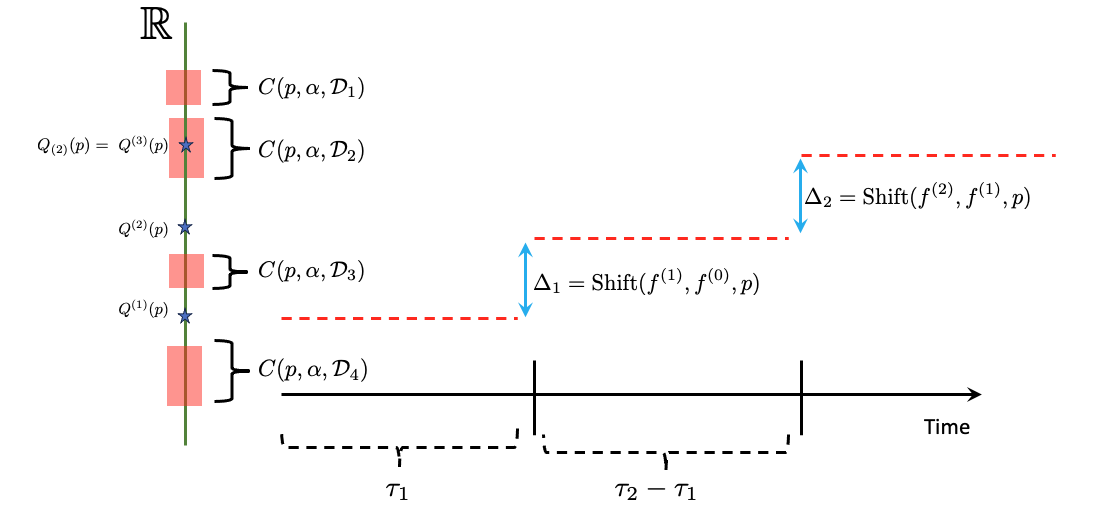
\includegraphics[width=0.9\linewidth]{anomaly/figs/separated_datasets.png}
%     \caption{An illustration of Assumption \ref{asumption_detectable} and \ref{defn:offline_datasets} on a stream with $2$ change-points ($H_T=2)$ and $K=4$ offline datasets. Assumption \ref{asumption_detectable} implies that the change-points on the stream are sufficiently far apart. Assumption \ref{defn:offline_datasets} implies that the $4$ CS do not intersect. Moreover, either the true quantile on the stream are outside the offline CS, i.e., $Q^{(1)}(p)$ and $Q^{(2)}(p)$ are not contained in any offline dataset's CS. Or, it is the case that the online quantile matches one of the offline dataset, i.e., $Q_{(2)}(p) = Q^{(3)}(p)$ in this example.}
%     \label{fig:separated_datasets_example}
% \end{figure}

}

\section{Proof for Theorem \ref{thm:core_theorem}, general case}
{\color{black}



To state performance guarantee of Algorithm \ref{alg:five}, we need a definition of a good event, which occurs with high probability.
\begin{definition}[Good event 4] 
Given a piece-wise stationary sequence $(S_t)_{t=1}^T := \Bigl(T,H_T, (\tau_c)_{c=0}^{H_T}, (f^{(c)})_{c=0}^{H_T}\Bigr)$, with the quantile functions of the $H_T+1$ different segments given by $(Q^{(c)}(\cdot))_{c=1}^{H_T}$ and $K$ offline datasets that are $(p,\alpha)$ separated according to Definition \ref{defn:offline_datasets}, let
% \begin{align}
% \begin{split}
%     \mathcal{E}_4 &:= \bigcap_{k=0}^{H_T} \bigcap_{s = \tau_{k}}^{\tau_{k+2}} \bigcap_{\tau'_k = s}^{\tau_{k+2}} \{ \Tilde{\theta}_{\tau_k:s} \in C_{\tau_k:s} \; \cap  \Tilde{\theta}_{s:\tau'_k} \in C_{s:\tau'_k}\}.\\
%     \end{split}

% \end{align}

\begin{align}
\begin{split}
    \gE_4 = \gG_2 \bigcap \underbrace{\bigcap_{p \in [0,1]}\bigcap_{j=1}^{K} \{ Q_{(k)}(p-u_{N_j}(\alpha)) \leq \widehat{Q}(p, \{ X_l^{(j)} \}_{l=1}^{N_j} ) \leq  Q_{(k)}(p+u_{N_j}(\alpha)) ) \}}_{\text{Offline dataset's CS contain true quantile}}   \\ \underbrace{\bigcap_{k=0}^{H_T}\bigcap_{t_1 = \tau_{k}}^{\tau_{k+1}} \bigcap_{t_2 = t_1 +1}^{\tau_{k+1}}   \bigg\{ \widehat{Q}(p-u_{t_2 - t_1}(\alpha), S_{t_1:t_2})  \leq Q^{(k)}(p) \leq \widehat{Q}(p-u_{t_2 - t_1}(\alpha), S_{t_1:t_2}) \bigg\}}_{\text{Online stream's CS contain true quantile}},
        \end{split}
                \label{eqn:good_event_4_defn}
\end{align}
where the $p$th quantile of the offline datasets $Q_{(l)}(p)$ are defined in Definition \ref{def:offline_quantile} and $\gG_2$ is defined in Equation (\ref{eqn:good_event_G}). 
\end{definition}

%
Event $\gE_4$ is the union of $\gE_2$ in Equation (\ref{eqn:good_event_2_defn}) for the online stream along with the event $\gE_3$ in Equation (\ref{eqn:good_event_3}) for the offline datasets. %The main result of this paper is stated below.

\begin{proposition}
    \begin{align*}
        \mathbb{P}[\gE_4] \geq 1- \alpha (K+2T)
    \end{align*}
    \label{prop:}
\end{proposition}
The proof follows similar to that of Proposition \ref{prop:good_event_2_prob}. 


%In this section, we specify the additional assumption on detectability, which combines the offline and online changes. 
As before, denote by $H_T$ as the number of change points, and the time-instants of change occuring at $1:= \tau_0 < \tau_1 < \tau_2 \cdots < \tau_{H_T} < \tau_{H_T+1}:= T+1$. We denote by the $k$th \emph{online stream} as the stationary samples $\{S_u : \tau_{k-1} \leq u < \tau_{k} \}$. 

For an offline dataset $j \in \{1,\cdots, K\}$ and the online stream $k$, $\Delta^{(j;k)} \geq 0$ denotes the shift between the $j$th offline dataset and the $k$th online stream. As before, similar to Theorem \ref{thm:online_shift}, for all $k \in [H_T]$, denote by $\Delta_{k} = \text{Shift} (f_{k},f_{k+1})$ to be the shift between the $k$th and $k-1$th online segment, and for $k \in [H_T]$ and $j \in [K]$, let $\Delta^{(j,k)} = \text{Shift} (f^{(k)},f_{(j)},p)$ be the shift between the $j$th offline dataset and the $k$th online segment. 
%The main detectability assumption in this section is the following which both Assumptions \ref{asumption_detectable} and \ref{as:offline_detectable}.

% \begin{assumption}[Offline assumption for every stream]
% We will assume that the number of offline dataset samples $N_1, \cdots, N_K$ and the number of online samples $(\tau_k - \tau_{k-1})_{k=1}^{H_T}$ satisfy  
% \begin{enumerate}
%     \item $\tau_{k} - \tau_{k-1} > D(\Delta_{k-1},\alpha) + D(\Delta_k, \alpha) + \max_{1 \leq j \leq K} D(\Delta^{(j;k)}, \alpha) \mathbf{1}(\Delta^{(j;k)} > 0)$
%     \item $N_j \geq \max_{1 \leq k \leq H_T} D(\Delta^{(j;k)}, \alpha) \mathbf{1}(\Delta^{(j;k)}>0)$
% \end{enumerate}
%     \label{as:offline_online_detect}
% \end{assumption}
% In words, the first assumption indicates that each stationary segment is large enough such that the change can be detected by using only the forward and backward confidence, and once a change is detected, the new segment can be matched with an offline dataset if the segment matches one of the offline datasets. The second assumption implies that if a given online segment's $p$th quantile is different from that of a offline dataset, then this change can be detected with high probability. 
% The detectability of this change is reliant on having sufficient number of samples in the offline dataset and thus the assumption is a lower bound on $N_j$. 
}

\begin{theorem*}[\ref{thm:core_theorem}] Let  $(S_t)_{t = 1}^T \sim \Bigl(T,H_T, (\tau_c)_{c=0}^{H_T}, (f_c)_{c=0}^{H_T}\Bigr)$  be a piece-wise stationary stream  satisfying Assumption \ref{asumption_detectable} and offline datasets  $\gD_1, \ldots, \gD_L$ satisfying  Assumption \ref{defn:offline_datasets}. Then, with probability at-least $1-(K+2T)\alpha$, for all times $T \in \mathbb{N}$, Algorithm \ref{alg:five} satisfies %{\em(i)} 
\begin{itemize}
    \item  $\text{FP} + \text{FN}  \leq \sum_{k=1}^{H_T} \left(D(\Delta_{k},\alpha) +  (1-\mathbf{1}_{\text{Match}_k})\max_{ j \in [K]} \left(\lceil \widehat{\tau}_j^{(k)}\rceil \mathbf{1}_{\text{Shift}(f^{(k)},f_{(j)},p) > 0}\right) \right)$ 
    \item Number of abstains less than 
    \begin{align*}
        \sum_{k=1}^{H_T} \Bigl[ &(1-\mathbf{1}_{\text{Match}_k}) 7 \sqrt{(\tau_k-\tau_{k-1}) \ln \left( \frac{1612}{\alpha^2} \ln(e(\tau_k-\tau_{k-1})) \right)}  \\ &+ \mathbf{1}_{\text{Match}_k}\left( 7 \sqrt{(N+T) \ln \left( \frac{1612\ln(e(N+T))}{\alpha^2} \right)}- 4 \sqrt{N \ln \left( \frac{1612\ln(eN)}{\alpha^2} \right)} \right) \\ &+  D(\Delta_{k},\alpha) +  \max_{ j \in [K]} \left(\lceil \widehat{\tau}_j^{(k)}\rceil \mathbf{1}_{\text{Shift}(f^{(k)},f_{(j)},p) > 0}\right)\Bigr],
    \end{align*}
\end{itemize}
where $\mathbf{1}_{\text{Match}_k} = \mathbf{1}_{Q^{(k)}(p) \in \{Q_{(1)}(p), \cdots, Q_{(K)}(p)\}}$, $Q^{(k)}(p)$ is the $p$th quantile of the $k$th segment of the online stream (Defn. \ref{def:piecewise}) and $Q_{(1)}(p), \cdots, Q_{(K)}(p)$ are the $p$th quantiles of the $K$ different offline datasets (Defn. \ref{definition:offline_dataset}).
\end{theorem*}




The proof structure follows a similar path as that of Theorem \ref{thm:online_shift}. Since Assumption \ref{asumption_detectable} holds, we know that Lemma \ref{lem:bdd_delay_change_induction} holds. Thus, we have that {\em(i)} there are no false positive change detections, and {\em(ii)} all changes are detected with a short detection delay. From the description of Algorithm \ref{alg:five}, we know that whenever a change is detected, a new instantiation of Algorithm \ref{alg:four} is started. Thus, the final result is obtained by summing the guarantees in Theorem \ref{thm:setting_3} over the $k$ online segments in addition to the delay taken to detect changes. 
The delay to detect changes are bounded by using Proposition \ref{prop:delay_bound} and Assumption \ref{asumption_detectable}, similar to that done in Theorem \ref{thm:online_shift}. 


% We will prove through induction, that under the good event $\mathcal{E}_4$ and Assumption \ref{as:offline_online_detect},  and {\em(iii)} if an online segment matches an offline dataset, then the match is identified quickly. If on the other hand a segment does not match any offline dataset, then the number of additional mistakes incurred is small. Concretely, the following is the key structural lemma of Algorithm \ref{alg:five}. 

% In order to state the lemma, we recall the notations that we set in the proof of Lemma \ref{lem:bdd_delay_change_induction}. As before, denote by $\tau_1 < \tau_2 \cdots < \tau_k < \tau_{k+1}$ be the set of times at which a true-change occurs. For each $k \in \{1, \cdots, H_T\}$, denote by $\tau_k^{'}$ as the time at which Algorithm \ref{alg:five} detects a change for the $k$th time.

% \begin{lemma}[No false change detections and bounded delay for identifying change and matching offline datasets]
%         Under the event $\mathcal{E}_4$, if Assumption \ref{as:offline_online_detect} holds, then for all $k \in \{1, \cdots, H_T\}$, 
%     \begin{itemize}
%         \item  $\tau_k^{'} \geq \tau_k$, and
%         \item $\tau_k^{'} - \tau_k \leq D(\Delta_k, \alpha)$.
%     \end{itemize}
%     \label{lem:bdd_delay_change_induction_general}
% \end{lemma}

% Before we prove the lemma, we show how this concludes the proof of Theorem \ref{thm:core_theorem}.

\begin{proof}[Proof of Theorem \ref{thm:core_theorem}]
    Theorem 6 is the joint result of theorems \ref{thm:online_shift} and \ref{thm:setting_3}. As in Theorem \ref{thm:online_shift}, Lemma \ref{lem:bdd_delay_change_induction} implies that at time $\tau'_k < \tau_{k+1}$, a new instantiation of Algorithm \ref{alg:four} is started. Theorem \ref{thm:setting_3} states that in the time interval $[\tau'_k, \tau_{k+1}]$, the $k$th online segment incurs a total number of mistakes bounded by the guarantee in Theorem \ref{thm:setting_3} for a time horizon $\tau_{k+1} - \tau'_{k}$. Concretely, in the time-interval $[\tau'_k, \tau_{k+1}]$, the sum of FP and FN is bounded above by $0$ in the event  $\mathbf{1}_{\text{Match}_k}$ holds, and by $\max_{ j \in [K]} \left(\lceil \widehat{\tau}_j^{(k)}\rceil \mathbf{1}_{\text{Shift}(f^{(k)},f_{(j)},p) > 0}\right) $ in the case when $\mathbf{1}_{\text{Match}_k}$ does not hold. %In other words, the sum of FP and FN in the time interval $\tau_{k+1} - \tau_{k}^{'}$ is at-most $\max_{1\leq j \leq K} D(\Delta^{(j;k)}, \alpha)\mathbf{1}(\Delta^{(j;k)} > 0)$. 
    Similarly, the number of abstains in the time-interval $\tau_{k+1} - \tau_{k}^{'}$ is given by the guarantee of Theorem \ref{thm:setting_3}. Now, summing over the $H_T$ different online segments yields the result. 
    
    For any segment $k \in [1, \ldots, H_T]$,  we have 
    \begin{itemize}
        \item $\text{FP}_k + \text{FN}_k  \leq D(\Delta_{k},\alpha) +   1-\mathbf{1}_{\text{Match}_k})\max_{ j \in [K]} \left(\lceil \widehat{\tau}_j^{(k)}\rceil \mathbf{1}_{\text{Shift}(f^{(k)},f_{(j)},p) > 0}\right)$ where the first term is from detection delay in detecting the change (Proposition \ref{prop:delay_bound}) and the second term from Theorem \ref{thm:setting_3}.
        \item If $Q^{(k)}(p)$ matches one of the dataset $\{Q_{(1)}(p), \cdots, Q_{(K)}(p)\}$, then under event $\gG_2$, number of abstains is at-most
        \begin{align*}
           D(\Delta_k, \alpha)+ \max_{ j \in [K]} \left(\lceil \widehat{\tau}_j^{(k)}\rceil \mathbf{1}_{\text{Shift}(f^{(k)},f_{(j)},p) > 0}\right) + 7 \sqrt{(N+\tau_k - \tau_{k-1}) \ln \left( \frac{1612\ln(e(N+\tau_k - \tau_{k-1}))}{\alpha^2} \right)} \\ - 7 \sqrt{N \ln \left( \frac{1612\ln(eN)}{\alpha^2} \right)},
        \end{align*}
        by Theorem \ref{thm:core_theorem}, case $\Delta = 0$.
        \item  If $Q^{(k)}(p)$ matches none of the datasets:
        \[ \text{Abstains} \leq   D(\Delta_k, \alpha)+ \max_{ j \in [K]} \left(\lceil \widehat{\tau}_j^{(k)}\rceil \mathbf{1}_{\text{Shift}(f^{(k)},f_{(j)},p) > 0}\right) + 7 \sqrt{(\tau_k - \tau_{k-1}) \ln \left( \frac{1612\ln(e(\tau_k - \tau_{k-1})))}{\alpha^2} \right)} 
        \]
        by theorem \ref{thm:core_theorem}, case $\Delta > 0$.
    \end{itemize}
The term of $D(\Delta_k, \alpha)$ always shows in all three equations above as that is the amount of time taken for the $k$th change-point to be detected and thus all decisions made during the times of change can potentially lead to mistakes and abstains. Combining the piece-wise results together, we have 
    \begin{align*}
    \text{FP} + \text{FN} \;  \leq \; & \sum_{k=1}^{H_T}D(\Delta_{k},\alpha) + (1-\mathbf{1}_{\text{Match}_k})  \max_{ j \in [K]} \left(\lceil \widehat{\tau}_j^{(k)}\rceil \mathbf{1}_{\text{Shift}(f^{(k)},f_{(j)},p) > 0}\right) 
        \end{align*}
        Similarly, summing over the $H_T$ online segments gives the bound on the number of abstains. 
         % \text{Abstains} \;  \leq \;  &  \sum_{k=1}^{H_t} \Bigl[ (1-\mathbf{1}_{\text{Match}_k}) \mathcal{O}(\sqrt{\tau_k - \tau_{k-1}}) \\ &+ \mathbf{1}_{\text{Match}_k}\left(\gO(\sqrt{N+(\tau_k-\tau_{k-1})} - \sqrt{N}) \right) \\ &+  D(\Delta_{k},\alpha) \Bigr],

\end{proof}

% --------------------------------------------------

% \subsection{Necessity of Assumption \ref{asumption_detectable}  }

% The core of our result requires that the changes are not too often, i.e., there is sufficient gap between changes, quantified precisely in Assumption \ref{asumption_detectable}. We remark that these assumptions are standard in the study of online decision making under non-stationarity \cite{liu2018change, JMLR:v23:20-1384}. This assumption ensures that all changes are detected. However, it is an interesting question to have a non-trivial analysis of dynamic decision making algorithms without assuming that each stationary environment is sufficiently long (Conclusion section of \cite{JMLR:v23:20-1384}). 

\section{Additional Related Works}
\label{app:related}

\paragraph{Online anomaly detection works} There exist works that focuses on other aspects of online anomaly detection. \cite{zhu2023meter} models online concept drift via an ensemble of models.   \cite{nardi2022anomaly} tackles modeling for online AD in a Federated setting. \cite{bhatia2022memstream} studies the low-memory constraint of online AD, and \cite{goyal2020drocc} focuses on efficiently modeling multi-dimensional data. A survey of methodologies of data modelling for AD can be found in the surveys of \cite{chandola2009anomaly, ruff2021unifying, pang2021deep}. Our work differs from these works in setting: we focus on dynamic thresholding of anomaly scores without having access or ability to retrain the underlying AD algorithm.

\paragraph{Threshold learning} Using score thresholds to make binary decision of seeking labels from human experts are studied in active learning \cite{balcan2007margin, zhang2016online,vishwakarma2023promises}. However, active learning does not have a concept of mistakes and is thus have different desiderata compared to our study. 

\section{Additional experiments and experiment details}
\label{app:exp1}

\subsection{Synthetic experiments}
We conduct our synthetic experiments for 1000 trails on streams each of length 1000. The normal distribution online streams are synthesized with parameters sampled uniformly form $[0, 10]$ for mean and $[0.2, 2]$ for variance. The Pareto distributions' parameters are sample uniformly from $[1,3]$ for $b$, $[0,10]$ for mean, and $[0.2,2]$ for scale. To synthesize distribution shifts, we sample a duration for each stationary piece from a Poisson distribution with $\lambda = 300$. To simulate datasets, we prepare $L=5$ offline datasets each of size $N=5000$; the online stream can be generated from either one of the dataset distributions or a random one with uniform probability. The range of these parameters are chosen to simulate real world anomaly score data. The code to generate the synthetic dataset as well as implementations of our algorithms will be open sourced.


\begin{table}[h!]
    \centering

    % \begin{tabular}{c c |c  c |c c}
    % \toprule
    %   & & \multicolumn{2}{|c|}{Normal} & \multicolumn{2}{|c}{Pareto} \\
    %   shift  & data   &  Abs. (\%) & Mis. (\%) &  Abs. (\%) & Mis. (\%)\\
    %   \midrule 
    %  x & x &  18.1 \plusminus{1.1} &  0 \plusminus{0} & 17.8 \plusminus{7.4} & .03 \plusminus{.01}\\
    %  \checkmark & x &   41.7 \plusminus{12.1} &  .05 \plusminus{0} &  51.9 \plusminus{35.0} & .51 \plusminus{.18}\\
    %  x & \checkmark  &  14.3 \plusminus{2.6} &  0 \plusminus{.01}& 16.8 \plusminus{4.7} & .06 \plusminus{.04} \\
    %  \checkmark  & \checkmark  & 32.9 \plusminus{7.1} &  .05 \plusminus{.03} & 24.3 \plusminus{5.2} &  .33 \plusminus{ .41 }\\
    % \bottomrule
    % \end{tabular}
    \begin{tabular}{c c |c c}
\toprule
  & & \multicolumn{2}{|c}{Pareto} \\
  shift & data & Abs. (\%) & Mis. (\%) \\
\midrule
 x & x & 17.8 \plusminus{7.4} & .03 \plusminus{.01} \\
 \checkmark & x & 51.9 \plusminus{35.0} & .51 \plusminus{.18} \\
 x & \checkmark & 16.8 \plusminus{4.7} & .06 \plusminus{.04} \\
 \checkmark & \checkmark & 24.3 \plusminus{5.2} & .33 \plusminus{.41} \\
\bottomrule
\end{tabular}

    \caption{Results of our algorithms on synthetic stream dataset generated from Pareto distribution.}
    \label{tab:synthetic_appendix}
\end{table}

\subsection{Case study of real AD application}
In this section we provide details on our real data experiments. We run Algorithms \ref{alg:two} and \ref{alg:five} on two large scale datasets {\ttfamily DS1} and {\ttfamily DS2} obtained from monitoring two large cloud computing services. Each dataset is a stream of anomaly scores obtained by applying a single anomaly detection algorithm. On these datasets, we run our two general algorithms, Algorithm \ref{alg:two} and \ref{alg:five} with $p = 1 - 10^{-6}$ and $\alpha = 10^{-6}$. Algorithm \ref{alg:five} can use offline datasets. In order to create them, we sampled 50 streams randomly that had length at-least $20,000$ in each of the two datasets. From this collection of $100$ streams, we sub-selected $37$ and $23$ streams from datasets {\ttfamily DS1} and {\ttfamily DS2} respectively such that no two datasets in this collection of $60$ streams overlapped. This is so that Assumption 6.1 is satisfied by the offline dataset. 

The description of the rest of the dataset on which we run the online algorithms is in Table \ref{tab:real_data_stats}. In addition, we also run {\ttfamily DSpot} \cite{siffer2017anomaly} with $p = 1 - 10^{-6}$ and set {\ttfamily num-init} to $500$ and {\ttfamily depth} to $100$ on the online algorithm dataset. All other parameters of {\ttfamily DSpot} was set to the suggested values in \cite{siffer2017anomaly}. In addition to these, we also compare against two static baselines of using the first $500$ and $100$ samples respectively and set the threshold as the max of the observed samples. This threshold is not changed since. 

The results of this experiment are reported in Table \ref{tab:real_data}. From this table, we can see that incorporating offline data reduces the number of abstains for both datasets without changing the volume of anomalies raised. This shows that when there are offline datasets available to the algorithm, the online performance is improved. 


\begin{table}[h!]
    \centering
    \begin{tabular}{c|c|c|c}
    \toprule
     & Num. of Streams & Average stream length &  Total num samples   \\ \midrule 
{DS1}  & $8377$ & $10925.4$ & $91521785$\\ \midrule
{DS2}  & $9657$ &  $10855.6$ & $104832532$\\
         \bottomrule
    \end{tabular}
    \caption{Summary of data properties for real world AD case study.}
    \label{tab:real_data_stats}
\end{table}


\begin{table}[h!]
    \centering

    \begin{tabular}{c|c|c|c| c| c|c}
    \toprule
                &  & Algo 3 & Algo 5 &  DSpot & $\tau^{(1)}$  & $\tau^{(2)}$  \\
        \midrule
         \multirow{2}{*}{DS1}  & Abstains $\downarrow$ & $13.6\%$ & $11.2\%$ & $1.2\%$ & $1.16\%$ & $0.05\%$\\
          & Anomaly $\downarrow$ & $\mathbf{.008\%}$ & {$\mathbf{.008\%}$} & $2.9\%$ & $0.02\%$ & $0.95\%$\\
          \midrule
         \multirow{2}{*}{DS2}  & Abstains $\downarrow$ & $13.3\%$ & $9.9\%$ & $1.3\%$& $1.25\%$ & $1.08\%$   \\
          & Anomaly $\downarrow$ & $.006\%$ & $\mathbf{.005\%}$ & $3.9\%$ & $0.07\%$ & $0.06\%$ \\
         \bottomrule
    \end{tabular}
    
    \caption{Case study performance. All baseline algorithms report anomaly rates much higher than the targeted $10^{-6}$, overwhelming the alarm system. By incorporating offline datasets, we are able to further decrease abstains and achieve a lower rate of reported anomaly. 
    }
    \label{tab:real_data}
\end{table}

\subsection{Additional experiment on open-source datasets}

We include additional experiments as follows. With the same underlying AD scoring algorithm (isolation forest for ForestCover, and a 3-layer MLP for Mammography), our confidence sequence algorithm (Algorithm \ref{alg:marginal_decision} in paper) can achieve a higher F1 score and fewer mistakes, with similar or less number of abstains, compared to a static threshold. This further demonstrates that our thresholding algorithm improves performance across datasets and base anomaly scoring algorithms.


\begin{table}[h!]
    \centering
    \begin{tabular}{ccc|cc}
        \toprule
       &\multicolumn{2}{c}{ForestCover (first 1500 as holdout)} & \multicolumn{2}{c}{Mammography (first 300 as holdout)} \\
        \midrule
        & Ours & Static Threshold & Ours & Static Threshold \\
        \midrule
        Abstain \% & 1.5\% & 1.5\% & 2.1\% & 5\% \\
        FP + FN & 645 & 1603 & 56 & 83 \\
        F1 & 0.39 & 0.33 & 0.51 & 0.43 \\
        \bottomrule
    \end{tabular}
    \caption{Performance comparison of algorithms on ForestCover and Mammography datasets}
    \label{tab:performance}
\end{table}



\section{Proof of Lower Bound}
\label{sec:lower_bound_proof}
The proof is based on the classical hypothesis testing lower bounds due to Neyman and Pearson. Throughout this section, we will fix a $T \in \mathbb{N}$ sufficiently large and let $\mathbb{P}_0 := N(0,1)$  be the standard normal distribution and $\mathbb{P}_{1} := N(\frac{1}{\sqrt{T}},1)$ as an unit variance normal distribution with mean $1/\sqrt{T}$. 

\begin{theorem}[Neyman-Pearson]
For any $T \in \mathbb{N}$, given $T$ i.i.d.. samples $S_{1:T}$, we want to distinguish between the two hypothesis $H_0: S_{1:T} \sim \mathbb{N}(0,1)$ or $H_1: S_{1:T} \sim \mathcal{N}(1/\sqrt{T},1)$. Then, for any measurable function $\mathcal{A} : \mathbb{R}^T \to \{0,1\}$, 
\begin{align*}
   \max( \mathbb{P}_0[\mathcal{A}(S_{1:T}=1], \mathbb{P}_0[\mathcal{A}(S_{1:T}=1]) \geq \frac{1}{4} \exp(-\frac{1}{2}),
\end{align*}
    where $\mathbb{P}_{i}$ for $i \in \{0,1\}$ is the proabability distribution under hypothesis $H_i$.
    \label{thm:neyman_pearson}
\end{theorem}

\begin{lemma}
    For every $p \in (0,1)$, there exists a constant $C_p \in (0,\infty)$ depending only on $p$, such that for $S \sim {N}(0,1)$
    \begin{align*}
        \mathbb{P}[S \in (Q^{(0)}(p), Q^{(1)}(p))] \geq \frac{C_p}{\sqrt{T}},
    \end{align*}
    where $Q^{(0)}(p)$ is the $p$th quantile of a $N(0,1)$ distribution and $Q^{(1)}(p)$ is the quantile of a $N(\frac{1}{\sqrt{T}},1)$ distribution.
    \label{lem:cp_lb}
\end{lemma}

Now, a standard Chernoff bound gives the following result.
\begin{lemma}[Chernoff bound]
Let $T \in \mathbb{N}$ and suppose $S_{1:T}$ are i.i.d., $N(0,1)$ random variables. Let $p \in (0,1)$. Then, 
\begin{align}
    \mathbb{P}\left[ \sum_{t=1}^T \mathbf{1}_{S_t \in (Q^{(0}(p), Q^{(1)}(p))} \leq \frac{C_p\sqrt{T}}{2} \right] \leq \exp \left( \frac{\sqrt{T}}{8} \right),
\end{align}
where $C_p$ is from Lemma \ref{lem:cp_lb}.
    \label{lem:lb_chernoff}
\end{lemma}

\begin{theorem}[Main lower bound]
Denote by two distributions  $\mathbb{P}_0 := N(0,1)$ and $\mathbb{P}_{1} := N(\frac{1}{\sqrt{T}},1)$ as unit variance guassians with means $0$ and $\frac{1}{\sqrt{T}}$ respectively. For $i \in \{0,1\}$, denote by $Q^{(i)}(p)$ as the $p$th quantile of distribution $\mathbb{P}_i$. For a threshold $\theta \in \mathbb{R}$ and sample $x \in \mathbb{R}$, denote by the indicator function $\widehat{Y}_t^{(\theta)}(x) := \mathbf{1}(x \geq \theta)$. Similarly, denote by the indicator function $Y_t^{(i)}(x) = \mathbf{1}(x \geq Q^{(i)})$ for $i \in \{0,1\}$. Let $\mathcal{A}: \mathbb{R}^T \to \{0,1\}$ be any measurable hypothesis testing function. Then, there exists $i \in \{0,1\}$ such that when $S_{1:T}$ are i.i.d. with distribution $\mathbb{P}_i$, then with probability at-least $\frac{1}{8} -  \exp \left( \frac{\sqrt{T}}{8} \right)$,
    \begin{align*}
 \sum_{t=1}^T \mathbf{1} ( \widehat{Y}_t^{(Q^{(\mathcal{A}(S_{1:T}))}(p))}(S_t) \neq Y_t^{(i)}(S_t) ) \geq C_p \sqrt{T},
    \end{align*}
where $C_p$ is from Lemma \ref{lem:cp_lb}.
    \label{thm:main_lower_bound}
\end{theorem}
In words, the above theorem states that even when the true distribution is known to be one of two possibilities and the optimal threshold is chosen using any measurable function, $O(\sqrt{T})$ mistakes is un-avoidable. 

\begin{proof}
Pick $\mathcal{A}: \mathbb{R}^T \to \{0,1\}$ by a measurable function that tests the hypothesis $H_0: S_{1:T}$ are i.i.d. with distribution $\mathbb{P}_0$ and $H_1: S_{1:T}$ are i.i.d. with distribution $\mathbb{P}_1$. From Theorem \ref{thm:neyman_pearson}, we know that for this given test $\mathcal{A}$, there exists $i \in \{0,1\}$ such that
\begin{align}
\mathbb{P}_i[\mathcal{A}(S_{1:T}) \neq i] \geq \frac{1}{8}.
\end{align}
Without loss of generality, lets suppose $i = 0$, i.e., given a hypothesis test $\mathcal{A}$, $\mathbb{P}_0[\mathcal{A}(S_{1:T}) \neq 0] \geq \frac{1}{8}$. We will show in the rest of the proof that for this $\mathcal{A}$, if $S_{1:T}$ are i.i.d. with distribution $\mathbb{P}_0$, $ \sum_{t=1}^T \mathbf{1} ( \widehat{Y}_t^{(Q^{(\mathcal{A}(S_{1:T}))}(p))} \neq Y_t^{(0)} ) \geq C_p \sqrt{T}$ holds with probability at-least $\frac{1}{8} -  \exp \left( \frac{\sqrt{T}}{8} \right)$.

To do so, let $S_{1:T}$ be i.i.d. $\mathbb{P}_0$. From Lemma \ref{lem:lb_chernoff}, we know that 
\begin{align*}
             \mathbb{P}_0\left[ \sum_{t=1}^T \mathbf{1}_{S_t \in (Q^{(0}(p), Q^{(1)}(p))} \leq \frac{C_p\sqrt{T}}{2} \right] \leq \exp \left( \frac{\sqrt{T}}{8} \right). 
\end{align*}
Thus, from an union bound, we know that for the given $\mathcal{A}$,
\begin{align*}
    \mathbb{P}_0 \left[ \underbrace{\mathcal{A}(S_{1:T}) \neq 0,  \sum_{t=1}^T \mathbf{1}_{S_t \in (Q^{(0}(p), Q^{(1)}(p))} \geq \frac{C_p\sqrt{T}}{2}  }_{\text{Event }\mathcal{H}}\right] \geq \frac{1}{8} - \exp \left( \frac{\sqrt{T}}{8} \right). 
\end{align*}

Observe that under event $\mathcal{H}$, for all $x \in \mathbb{R}$, we have the equality

\begin{align*}
     \mathbf{1} ( \widehat{Y}_t^{(\mathcal{A}(S_{1:T}))}(x) \neq Y_t^{(0)}(x) ) = \mathbf{1} (x \in (Q^{(0)}(p), Q^{(1)}(p)).
\end{align*}
Thus, under event $\mathcal{H}$, we have 
\begin{align*}
    \sum_{t=1}^T \mathbf{1} ( \widehat{Y}_t^{(\mathcal{A}(S_{1:T}))}(S_t) \neq Y_t^{(0)}(S_t) ) = \sum_{t=1}^T \mathbf{1}_{S_t \in (Q^{(0}(p), Q^{(1)}(p))} \geq \frac{C_p\sqrt{T}}{2},
\end{align*}
holding with probability at-least $\frac{1}{8} - \exp \left( \frac{\sqrt{T}}{8} \right).$
\end{proof}

%\subsection{Discussion of the lower bound}

The theorem asserts that if an algorithm does not abstain, then even in a stationary stream, $O(\sqrt{T})$ mistakes will occur with high probability. 


%\bibliographystyle{plain}
%\bibliography{ref}
